\documentclass[11pt,a4paper]{article}

\usepackage[T1]{fontenc}
\usepackage[utf8]{inputenc}
\usepackage{amsmath,amsthm}
\usepackage{newtxtext,newtxmath}
\usepackage[varqu]{zi4}
\usepackage{microtype}
\usepackage[margin=1in]{geometry}
\usepackage{array,booktabs,tabularx}
\usepackage[dvipsnames]{xcolor}
\usepackage{tikz}
\usetikzlibrary{positioning,arrows.meta,shapes.geometric,calc,fit,backgrounds,decorations.pathreplacing}
\usepackage{pgfplots}
\pgfplotsset{compat=1.18}
\usepackage{listings}
\usepackage[most]{tcolorbox}
\usepackage[font=small,labelfont=bf]{caption}
\usepackage{enumitem}
\usepackage[colorlinks,linkcolor=MidnightBlue,citecolor=MidnightBlue,urlcolor=MidnightBlue]{hyperref}
\usepackage[nameinlink]{cleveref}

% ---------------------------------------------------------------- notation
\newcommand{\ap}{\mathtt{@}}
\newcommand{\cl}[2]{\langle #1,\, #2\rangle}
\newcommand{\emp}{[\,]}
\newcommand{\rul}[1]{\textsc{#1}}
\newcommand{\ins}[1]{\textsf{#1}}
\newcommand{\sem}[1]{[\![#1]\!]}
\newcommand{\trans}{\;\longrightarrow\;}
\newcommand{\Real}{\mathit{Real}}
\newcommand{\st}[4]{(#1,\ #2,\ #3,\ #4)}

\definecolor{sfill}{HTML}{DCE9F7}
\definecolor{efill}{HTML}{DDF0DC}
\definecolor{cfill}{HTML}{FCE8D2}
\definecolor{dfill}{HTML}{F1DDEE}
\definecolor{sline}{HTML}{2F6DB5}
\definecolor{eline}{HTML}{3C8A3A}
\definecolor{cline}{HTML}{C7701C}
\definecolor{dline}{HTML}{9A3F8E}

\tikzset{
  >=Stealth,
  every picture/.append style={font=\small},
  cellb/.style={draw, minimum height=0.6cm, minimum width=0.7cm, inner sep=2pt, fill=white},
  ptr/.style={->, thick},
  regbox/.style={draw=#1, thick, rounded corners=3pt, align=center, minimum width=2.8cm, minimum height=1.7cm},
}

\theoremstyle{definition}
\newtheorem{definition}{Definition}
\newtheorem{exercise}{Exercise}
\theoremstyle{plain}
\newtheorem{theorem}{Theorem}

\newtcolorbox{aside}[1]{enhanced, breakable, colback=black!3, colframe=black!35,
  boxrule=0.5pt, arc=2pt, fonttitle=\bfseries\small, title={#1}, coltitle=black,
  colbacktitle=black!10, left=6pt, right=6pt}

\lstset{language=C, basicstyle=\ttfamily\small, keywordstyle=\bfseries,
  commentstyle=\color{black!55}, columns=fullflexible, keepspaces,
  frame=single, rulecolor=\color{black!30}, xleftmargin=6pt, xrightmargin=6pt,
  aboveskip=8pt, belowskip=8pt, tabsize=8}

\title{The SECD Machine\\[4pt]\large A Tutorial Introduction}
\author{}
\date{\today}

\begin{document}
\maketitle

\begin{abstract}
\noindent
The SECD machine, introduced by Peter Landin in 1964, was the first abstract
machine for evaluating expressions of the $\lambda$-calculus, and it remains the
standard first example of how a functional language can be implemented.
This tutorial builds the machine up from three ideas: replacing substitution by
\emph{environments}, representing functions as \emph{closures}, and making the
evaluator's own call stack explicit as the \emph{dump}.
We give the transition rules, trace several programs step by step, state what
the machine computes, and program it with Church encodings up to a recursive
factorial. We then look inside a small C implementation, including a
pointer-sharing bug that is instructive in its own right, and show how the
machine turns into a compiler target. A section on related machines and a set
of exercises close the paper. The only prerequisite is a working knowledge of
the untyped $\lambda$-calculus.
\end{abstract}

\tableofcontents

% =====================================================================
\section{Introduction}

A $\lambda$-term on paper is evaluated by \emph{rewriting}: find a redex
$(\lambda x.M)\,N$, replace it by $M[N/x]$, and repeat. This is a fine
mathematical definition, but it is a poor description of what a computer does.
Each step has to search the term for the next redex, copy $N$ into every
occurrence of $x$, and rename bound variables to avoid capture. None of this
resembles running a program, where code is fixed, data lives in memory, and a
stack records what to do after a function returns.

An \emph{abstract machine} closes that gap. It is a state-transition system whose
states are made of simple data structures (stacks, lists, tables) and whose
transitions each do a small, bounded amount of work. It sits between the
mathematical semantics, which says \emph{what} a term means, and a real
implementation, which says \emph{how} the bits move.

Landin's SECD machine~\cite{landin64} was the first such machine for the
$\lambda$-calculus. Its name lists its four registers:
\begin{center}
\begin{tabular}{@{}ll@{}}
\textbf{S}tack & values computed so far, waiting to be used;\\
\textbf{E}nvironment & the values of the variables currently in scope;\\
\textbf{C}ontrol & the expressions still to be evaluated;\\
\textbf{D}ump & saved copies of S, E and C, to resume after a function returns.
\end{tabular}
\end{center}
By the end of this tutorial you should be able to run the machine by hand,
explain why each register is needed, read and modify an implementation, and
recognise the SECD machine's ideas in the implementations of real languages.

\paragraph{Companion code.}
The examples are executed by a short C program, \texttt{secd23.c}, which
follows the presentation of Field and Harrison~\cite{fieldharrison}. All
traces, step counts and the plot in \cref{sec:programming} were produced by
running it. \Cref{sec:implementation} walks through the program.

% =====================================================================
\section{What we assume}\label{sec:background}

We use the untyped $\lambda$-calculus with the usual conventions: application
associates to the left, so $M\,N\,P$ means $(M\,N)\,P$, and the body of a
$\lambda$ extends as far right as possible.
\[
  M, N ::= x \;\mid\; \lambda x.M \;\mid\; M\,N
\]
A term may contain free variables. We treat these as names of
\emph{constants} supplied from outside, for example $x = 4$ and $y = 3$. This
lets the examples produce readable results without first adding numbers
to the language.

\paragraph{Call-by-value.}
The SECD machine implements \emph{call-by-value} evaluation. The
\emph{values} are $\lambda$-abstractions and constants. An application
$M\,N$ is evaluated by evaluating both $M$ and $N$ to values and then, if the
function is $\lambda x.B$ and the argument is $V$, continuing with $B[V/x]$.
Two consequences matter throughout:
\begin{enumerate}[nosep]
\item Arguments are evaluated \emph{before} the call, even if the function
  never uses them. If the argument diverges, the whole call diverges.
\item Evaluation stops at a $\lambda$. We never evaluate inside the body of a
  function that has not been called. The term $\lambda b.(\lambda z.z)\,4$ is
  already a value. A term in this state, with no redex outside any $\lambda$,
  is said to be in \emph{weak head normal form} (WHNF)%
  \footnote{Strictly, the C program's tag name \texttt{WHNF} covers all the
  machine's values. For call-by-value these are exactly the closures and
  constants.}.
\end{enumerate}

\paragraph{A running example.}
Let $K = \lambda a.\lambda b.a$. With $x=4$ and $y=3$, call-by-value
evaluation by substitution goes
\begin{equation}\label{eq:ksub}
  K\,x\,y \;=\; (\lambda a.\lambda b.a)\,4\,3
  \;\to\; (\lambda b.4)\,3
  \;\to\; 4 .
\end{equation}
We will run the same computation on the machine in \cref{sec:examples} and
see each of these two $\beta$-steps reappear in a different form.

% =====================================================================
\section{From substitution to a machine}\label{sec:ideas}

The machine is built from three ideas. Each one fixes a specific problem with
evaluation by rewriting.

\subsection{Environments instead of substitution}

Substitution $B[V/x]$ copies $V$ into the body $B$, and so creates a new term
at every call. The alternative is to leave $B$ untouched and remember, in a
separate table, that $x$ now stands for $V$. When evaluation later meets
$x$, it looks the value up. This table is the \emph{environment}.

We write an environment as a list of bindings, most recent first, such as
$E_0 = [x \mapsto 4,\ y \mapsto 3]$. Extending an environment adds a binding at
the front:
\[
  E_0[a\mapsto 4] = [a\mapsto 4,\ x\mapsto 4,\ y\mapsto 3].
\]
Lookup searches from the front, so a newer binding of a name \emph{shadows}
an older one. Because extension only adds a new cell in front of an existing
list, the old list is shared rather than copied. Environments created by
different calls therefore form a tree of linked cells
(\cref{fig:heap,fig:lexical}).

\subsection{Closures: functions carry their environment}

With environments a new problem appears. Suppose a $\lambda$-term is
evaluated, passed somewhere else, and called later. Its body may refer to
variables that were in scope where the $\lambda$ was \emph{written}. By the
time it is called, the environment in force may have changed. Consider
\begin{equation}\label{eq:lexical}
  T \;=\; (\lambda f.\,(\lambda x.\,f\,x)\;y)\;(\lambda z.\,x)
  \qquad\text{in } E_0 = [x\mapsto 4,\ y\mapsto 3].
\end{equation}
The function $\lambda z.x$ is created where $x = 4$. It is called inside
$\lambda x.f\,x$, where $x$ has been rebound to $y = 3$. Substitution gives
\[
  T \to (\lambda x.\,(\lambda z.4)\,x)\;3 \to (\lambda z.4)\,3 \to 4,
\]
so the $x$ in $\lambda z.x$ must mean the $x$ that was visible \emph{where the
function was written}. This rule is called \emph{lexical} (or \emph{static})
scoping. To get it without substitution, a function value must remember the
environment it was created in. The pair
\[
  \cl{\lambda x.B}{E}
\]
of a $\lambda$-term and an environment is called a \emph{closure}. When the
closure is called with argument $v$, its body $B$ runs in $E[x\mapsto v]$:
the closure's \emph{own} environment extended with the parameter, rather than
the caller's environment.

Using the caller's environment instead is called \emph{dynamic} scoping, and
for $T$ it would give $3$. Early Lisp systems behaved that way, which is
known as the \emph{funarg problem}. Landin's closures were the fix.
\Cref{fig:lexical} shows the environments involved in evaluating $T$.

\begin{figure}[t]
\centering
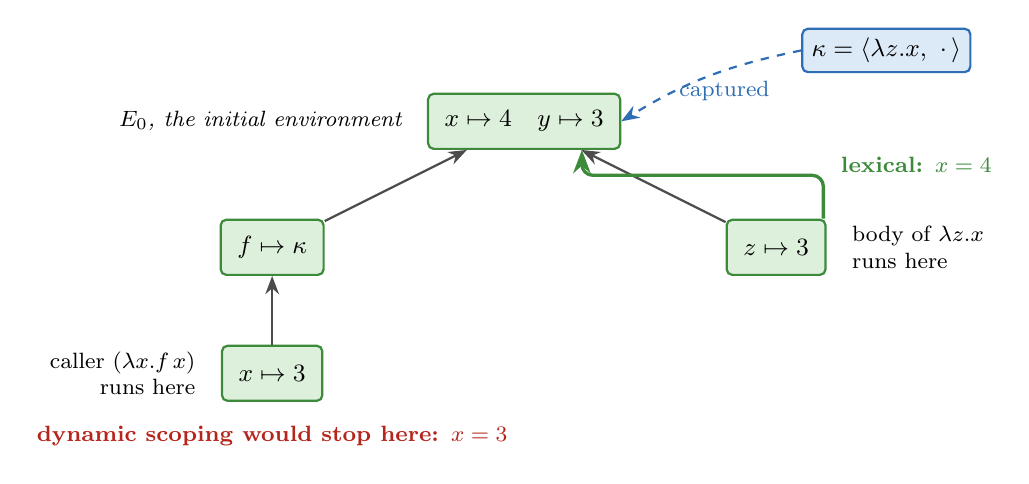
\begin{tikzpicture}[
  env/.style={draw=eline, thick, fill=efill, rounded corners=2pt, minimum height=0.7cm, inner xsep=6pt},
  up/.style={->, thick, black!70},
]
\node[env] (E0) at (0,0) {$x\mapsto 4\quad y\mapsto 3$};
\node[env] (Ef) at (-3.2,-1.6) {$f\mapsto\kappa$};
\node[env] (Ex) at (-3.2,-3.2) {$x\mapsto 3$};
\node[env] (Ez) at (3.2,-1.6) {$z\mapsto 3$};
\node[draw, thick, rounded corners=2pt, fill=sfill, draw=sline] (k) at (4.6,0.9) {$\kappa = \cl{\lambda z.x}{\,\cdot\,}$};
\node[left=2mm of E0, font=\footnotesize\itshape] {$E_0$, the initial environment};
\draw[up] (Ef) -- (E0);
\draw[up] (Ex) -- (Ef);
\draw[up] (Ez) -- (E0);
\draw[->, thick, dashed, sline] (k.west) to[bend right=10] node[below, font=\footnotesize, pos=0.4] {captured} (E0.east);
\node[right=2mm of Ez, align=left, font=\footnotesize] {body of $\lambda z.x$\\ runs here};
\node[left=2mm of Ex, align=right, font=\footnotesize] {caller $(\lambda x.f\,x)$\\ runs here};
% lexical lookup
\draw[->, very thick, eline, rounded corners] ($(Ez.north)+(0.6,0)$) -- ++(0,0.55) -| ($(E0.south east)+(-0.5,0)$);
\node[eline, font=\footnotesize\bfseries, anchor=west] at (3.9,-0.55) {lexical: $x = 4$};
% dynamic lookup
\node[BrickRed, font=\footnotesize\bfseries] at (-3.2,-4.0) {dynamic scoping would stop here: $x = 3$};
\end{tikzpicture}
\caption{Environments while evaluating $T$ from \eqref{eq:lexical}. Arrows
point from each environment to the older one it extends. The closure $\kappa$
for $\lambda z.x$ captured $E_0$. When $\kappa$ is called with $3$, its body
runs in $[z\mapsto 3]$ extending $E_0$ (right branch), so looking up $x$ finds
$4$. The caller's environment (left branch) is never consulted.}
\label{fig:lexical}
\end{figure}

\subsection{Control and stack: evaluation as postfix code}

How does the machine decide what to evaluate next? Think of a pocket
calculator evaluating $2\times(3+4)$. The expression is a tree, but a stack
calculator receives it in \emph{postfix} order, $2\ 3\ 4\ {+}\ {\times}$:
numbers are pushed onto a stack, and an operator pops its operands and pushes
the result (\cref{fig:rpn}).

\begin{figure}[t]
\centering
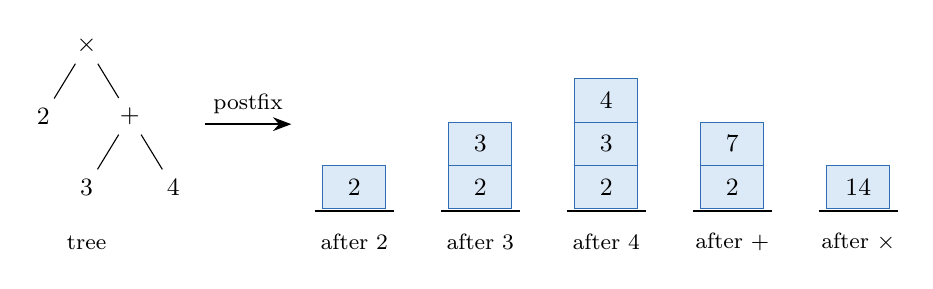
\begin{tikzpicture}[
  scell/.style={draw=sline, fill=sfill, minimum width=0.8cm, minimum height=0.55cm},
  level distance=0.9cm, sibling distance=1.1cm,
  every node/.append style={font=\small}]
\node (t) at (-3.4,1.4) {$\times$}
  child {node {$2$}}
  child {node {$+$} child {node {$3$}} child {node {$4$}}};
\node[font=\footnotesize] at (-3.4,-1.1) {tree};
\draw[->, thick] (-1.9,0.4) -- node[above, font=\footnotesize] {postfix} (-0.8,0.4);
\foreach \i/\items/\tok in {0/{2}/2, 1/{2,3}/3, 2/{2,3,4}/4, 3/{2,7}/+, 4/{14}/{\times}} {
  \foreach \v [count=\k from 0] in \items {
    \node[scell] at (1.6*\i, 0.55*\k - 0.4) {$\v$};
  }
  \node[font=\footnotesize] at (1.6*\i, -1.1) {after $\tok$};
  \draw[thick] (1.6*\i - 0.5, -0.7) -- (1.6*\i + 0.5, -0.7);
}
\end{tikzpicture}
\caption{A stack calculator evaluating $2\times(3+4)$. The tree is flattened
into postfix order. Constants are pushed, and operators replace their operands
by the result. The SECD machine does the same with application in place of
$+$ and $\times$, and the marker $\ap$ playing the role of the operator.}
\label{fig:rpn}
\end{figure}

The SECD machine works the same way. The \emph{control} C is the list of
things still to be done, and the \emph{stack} S holds the values produced so
far. Function application plays the role of the operator. To evaluate
$M\,N$, the machine replaces it on the control by the sequence
\[
  N,\ M,\ \ap
\]
That is: evaluate the argument, evaluate the function, then apply. The
marker $\ap$ (``apply'') is the machine's only operator symbol, and Landin
wrote it $\mathit{ap}$. When $\ap$ reaches the front of the control, the
function and its argument are the top two values on the stack.

Unlike the calculator, the machine flattens the tree \emph{lazily}, one
application node at a time, as each node reaches the front of the control.
\Cref{sec:compiling} shows that flattening the whole tree in advance turns
the machine into a compiler target.

\subsection{The dump: an explicit call stack}

The last ingredient deals with function calls. When a closure
$\cl{\lambda x.B}{E'}$ is applied, its body $B$ must run with a fresh stack, in
the environment $E'[x\mapsto v]$, with $B$ as the control. Afterwards the
machine has to return to exactly where it was: the old stack (minus the
function and argument), the old environment, and the rest of the old control.

The \emph{dump} D saves that triple $(S, E, C)$. A call pushes a triple onto
the dump, and when the body's control runs out the machine pops it back. The
dump is the machine's call stack, and each triple is an activation record.
In modern terms it represents the \emph{continuation}, everything that
remains to be done once the current call finishes~\cite{danvy-secd}.

A recursive evaluator, written as an ordinary program, gets this bookkeeping for
free from the call stack of the language it is written in. The point of
the dump is to make that hidden stack visible as data. Every transition is then
a constant amount of work, with nothing hidden in the implementation language.

% =====================================================================
\section{The machine}\label{sec:machine}

\subsection{States}

\begin{definition}[SECD state]
A \emph{state} is a quadruple $\st{S}{E}{C}{D}$ where
\begin{itemize}[nosep]
\item $S$ is a list of values (top first). A value is a constant, a
  primitive function, or a closure $\cl{\lambda x.B}{E}$;
\item $E$ is an environment, a list of bindings $x\mapsto v$;
\item $C$ is a list of control items. Each is either a $\lambda$-term or the
  marker $\ap$;
\item $D$ is a list of saved triples $(S', E', C')$.
\end{itemize}
\end{definition}

We write $v : S$ for the list with head $v$ and tail $S$, $\emp$ for the
empty list, and $[v_1, \dots, v_n]$ for short lists.
\Cref{fig:overview} pictures a state.

\begin{figure}[t]
\centering
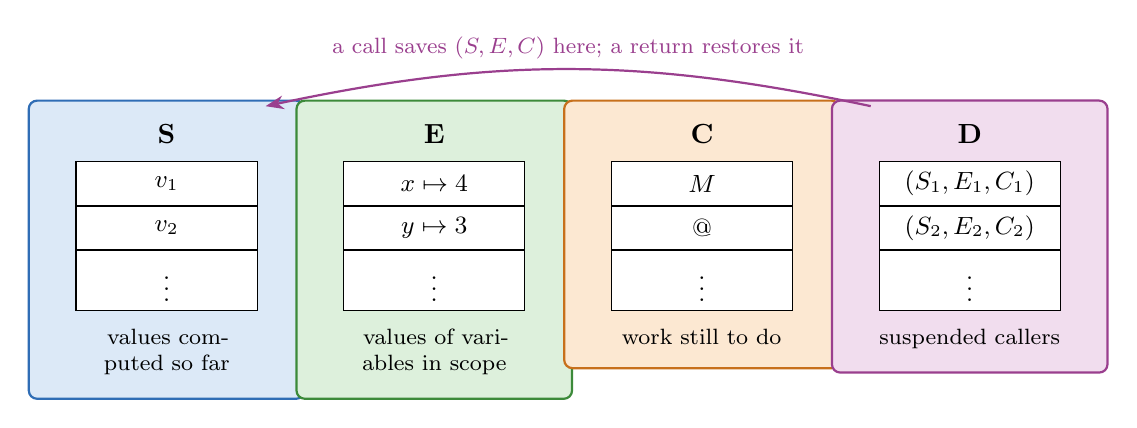
\begin{tikzpicture}[
  c/.style={draw, minimum width=2.3cm, minimum height=0.55cm, fill=white},
  title/.style={font=\bfseries},
  note/.style={font=\footnotesize, align=center, text width=2.9cm},
]
\foreach \x/\name/\col/\fillc/\a/\b/\c/\note in {
   0/S/sline/sfill/{$v_1$}/{$v_2$}/{$\vdots$}/{values computed so far},
   3.4/E/eline/efill/{$x\mapsto 4$}/{$y\mapsto 3$}/{$\vdots$}/{values of variables in scope},
   6.8/C/cline/cfill/{$M$}/{$\ap$}/{$\vdots$}/{work still to do},
   10.2/D/dline/dfill/{$(S_1,E_1,C_1)$}/{$(S_2,E_2,C_2)$}/{$\vdots$}/{suspended callers}} {
  \node[c] (\name1) at (\x,0) {\a};
  \node[c, below=0pt of \name1] (\name2) {\b};
  \node[c, below=0pt of \name2] (\name3) {\c};
  \node[title, above=3pt of \name1] (\name t) {\name};
  \node[note, below=3pt of \name3] (\name n) {\note};
  \begin{scope}[on background layer]
    \node[draw=\col, thick, fill=\fillc, rounded corners=3pt, inner sep=5pt, fit=(\name t)(\name1)(\name3)(\name n)] {};
  \end{scope}
}
\draw[->, thick, dline] ($(D1.north west)+(-0.1,0.7)$) to[bend right=12]
  node[above, font=\footnotesize, pos=0.5] {a call saves $(S,E,C)$ here; a return restores it}
  ($(S1.north east)+(0.1,0.7)$);
\end{tikzpicture}
\caption{The four registers of the SECD machine. Each is a list, drawn with
its head at the top. The dump holds complete copies of the other three
registers, one per pending call.}
\label{fig:overview}
\end{figure}

\subsection{Transitions}

The transition rules are given in \cref{fig:rules}. Each rule looks only at
the head of the control (or, when the control is empty, at the dump). Exactly
one rule applies to any state that is not final or stuck. We name the rules,
and the C program labels them with the case numbers in parentheses.

\begin{figure}[t]
\begin{tcolorbox}[colback=white, colframe=black!40, boxrule=0.6pt, arc=2pt, left=2pt, right=2pt]
\small
\[
\begin{array}{@{}l@{\quad}r@{\;}c@{\;}l@{}}
\rul{Var}\ (1a) &
  \st{S}{E}{x : C}{D} &\longrightarrow& \st{E(x) : S}{E}{C}{D}\\[6pt]
\rul{Abs}\ (1b) &
  \st{S}{E}{\lambda x.B : C}{D} &\longrightarrow& \st{\cl{\lambda x.B}{E} : S}{E}{C}{D}\\[6pt]
\rul{App}\ (1c) &
  \st{S}{E}{(M\,N) : C}{D} &\longrightarrow& \st{S}{E}{N : M : \ap : C}{D}\\[6pt]
\rul{Call}\ (1d\,ii) &
  \st{\cl{\lambda x.B}{E'} : v : S}{E}{\ap : C}{D} &\longrightarrow&
  \st{\emp}{E'[x\mapsto v]}{[B]}{(S,E,C) : D}\\[6pt]
\rul{Prim}\ (1d\,i) &
  \st{f : v : S}{E}{\ap : C}{D} &\longrightarrow& \st{\delta(f,v) : S}{E}{C}{D}\\[6pt]
\rul{Return}\ (2) &
  \st{v : S}{E}{\emp}{(S',E',C') : D} &\longrightarrow& \st{v : S'}{E'}{C'}{D}
\end{array}
\]
\par\medskip
\textbf{Start:} $\st{\emp}{E_0}{[M]}{\emp}$ evaluates $M$ with free
variables bound by $E_0$.\quad
\textbf{Halt:} $\st{v : S}{E}{\emp}{\emp}$; the result is $v$.\\
\textbf{Stuck:} \rul{Var} with $x$ unbound, or $\ap$ with a constant in
function position.\quad
\rul{Prim} applies when $f$ is a primitive; $\delta$ is its meaning (\cref{sec:primitives}).
\end{tcolorbox}
\caption{The transition rules of the SECD machine.}
\label{fig:rules}
\end{figure}

In words:
\begin{description}[style=nextline, leftmargin=1.2em, itemsep=2pt]
\item[\rul{Var}] A variable is evaluated by looking it up. Its value goes on
  the stack.
\item[\rul{Abs}] A $\lambda$ is already a value, but it must remember the
  current environment, so the machine pushes a closure. The body is
  \emph{not} evaluated. This is where the machine stops at WHNF.
\item[\rul{App}] An application is split into its parts, with the marker $\ap$
  scheduled after both (\cref{fig:app}). Note the order: the argument $N$ is
  evaluated \emph{first}, so that when $\ap$ comes up the function is on top
  of the stack and the argument just below it. This right-to-left order is the
  one used by Landin and by the C program. For pure terms that terminate, the
  order does not change the result.
\item[\rul{Call}] The function is a closure. The machine saves the current
  stack, environment and control on the dump, then starts the body in the
  closure's environment extended with the argument (\cref{fig:callret}, top).
\item[\rul{Return}] The control is empty, so the current body has finished
  with its result on top of the stack. The machine pops the saved triple and
  pushes the result onto the restored stack (\cref{fig:callret}, bottom).
\end{description}

\begin{figure}[t]
\centering
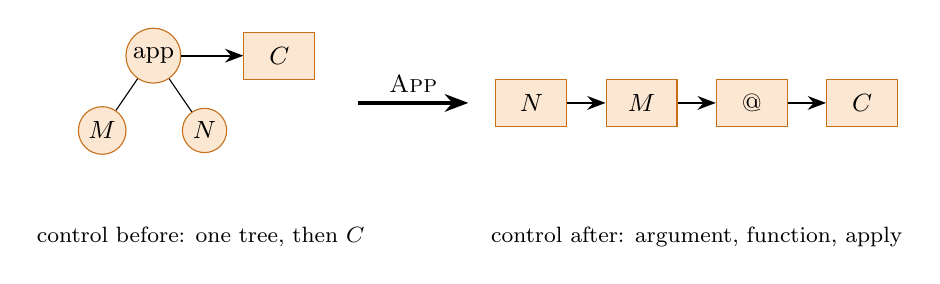
\begin{tikzpicture}[level distance=0.95cm, sibling distance=1.3cm,
  ccell/.style={draw=cline, fill=cfill, minimum width=0.9cm, minimum height=0.6cm}]
\node[draw=cline, fill=cfill, circle, inner sep=1.5pt] (r) at (0,0) {app}
  child {node[draw=cline, fill=cfill, circle, inner sep=2pt] {$M$}}
  child {node[draw=cline, fill=cfill, circle, inner sep=2pt] {$N$}};
\node[ccell] (rest0) at (1.6,0) {$C$};
\draw[ptr] (r) -- (rest0);
\node[font=\footnotesize] at (0.6,-2.3) {control before: one tree, then $C$};
\draw[-{Stealth[length=3mm]}, line width=1.2pt] (2.6,-0.6) -- node[above] {\rul{App}} (4.0,-0.6);
\node[ccell] (n) at (4.8,-0.6) {$N$};
\node[ccell] (m) at (6.2,-0.6) {$M$};
\node[ccell] (a) at (7.6,-0.6) {$\ap$};
\node[ccell] (rest) at (9.0,-0.6) {$C$};
\draw[ptr] (n) -- (m); \draw[ptr] (m) -- (a); \draw[ptr] (a) -- (rest);
\node[font=\footnotesize, align=center] at (6.9,-2.3) {control after: argument, function, apply};
\end{tikzpicture}
\caption{\rul{App} replaces one application node by three control items.
This is one step of the postfix flattening from \cref{fig:rpn}.}
\label{fig:app}
\end{figure}

\begin{figure}[t]
\centering
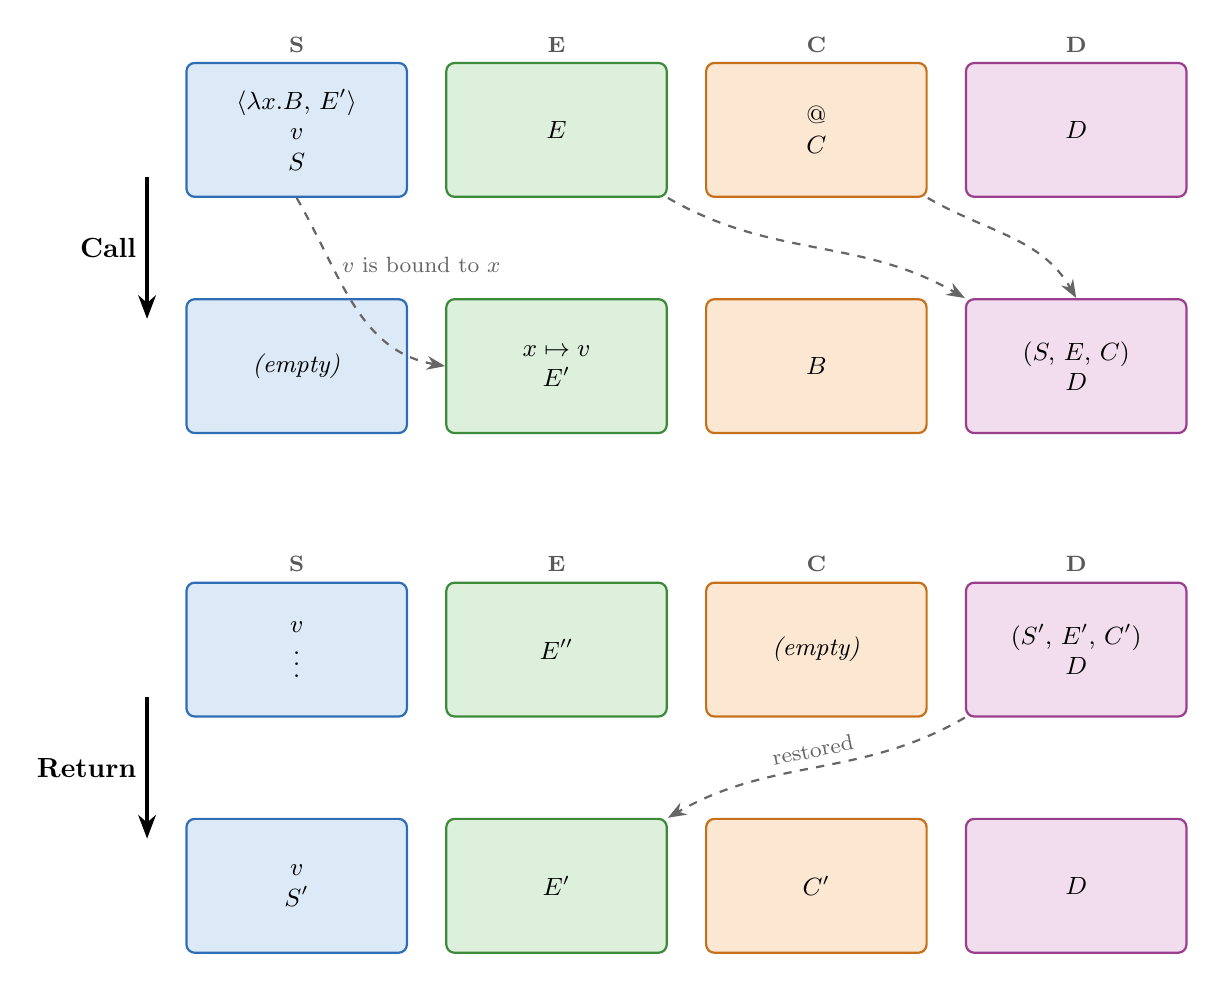
\begin{tikzpicture}[
  lab/.style={font=\footnotesize\bfseries, text=black!65}]
\newcommand{\staterow}[7]{%
  \node[regbox=sline, fill=sfill] (#1S) at (0,#2) {#3};
  \node[regbox=eline, fill=efill] (#1E) at (3.3,#2) {#4};
  \node[regbox=cline, fill=cfill] (#1C) at (6.6,#2) {#5};
  \node[regbox=dline, fill=dfill] (#1D) at (9.9,#2) {#6};
  \ifx#7y\foreach \r in {S,E,C,D} {\node[lab, above=0pt of #1\r] {\r};}\fi
}
% ---- call
\staterow{a}{0}{$\cl{\lambda x.B}{E'}$\\ $v$\\ $S$}{$E$}{$\ap$\\ $C$}{$D$}{y}
\staterow{b}{-3.0}{\textit{(empty)}}{$x\mapsto v$\\ $E'$}{$B$}{$(S,\,E,\,C)$\\ $D$}{n}
\draw[-{Stealth[length=3mm]}, line width=1.2pt] (-1.9,-0.6) -- node[left, font=\bfseries] {\rul{Call}} (-1.9,-2.4);
\draw[->, thick, dashed, black!60] (aS.south) to[out=-60, in=170] node[pos=0.3, right, font=\footnotesize] {$v$ is bound to $x$} (bE.west);
\draw[->, thick, dashed, black!60] (aE.south east) to[out=-30, in=150] (bD.north west);
\draw[->, thick, dashed, black!60] (aC.south east) to[out=-30, in=120] (bD.north);
% ---- return
\staterow{c}{-6.6}{$v$\\ $\vdots$}{$E''$}{\textit{(empty)}}{$(S',\,E',\,C')$\\ $D$}{y}
\staterow{d}{-9.6}{$v$\\ $S'$}{$E'$}{$C'$}{$D$}{n}
\draw[-{Stealth[length=3mm]}, line width=1.2pt] (-1.9,-7.2) -- node[left, font=\bfseries] {\rul{Return}} (-1.9,-9.0);
\draw[->, thick, dashed, black!60] (cD.south west) to[out=-150, in=30] node[pos=0.5, above, font=\footnotesize, sloped] {restored} (dE.north east);
\end{tikzpicture}
\caption{Calling and returning. \textbf{Top:} \rul{Call} consumes the closure
and its argument, saves the rest of the state on the dump, and starts the body
$B$ on an empty stack in the closure's environment. \textbf{Bottom:} when the
body's control is used up, \rul{Return} restores the saved state and pushes the
result $v$ onto it. Note that the closure's environment $E'$, not the caller's
$E$, is what the body sees.}
\label{fig:callret}
\end{figure}

\subsection{The machine as a loop}

\Cref{fig:loop} shows the transition rules as the control flow of an
interpreter's main loop, which is how the C program is organised. Each pass
through the loop performs exactly one transition. The loop ends when the
control and the dump are both empty.

\begin{figure}[t]
\centering
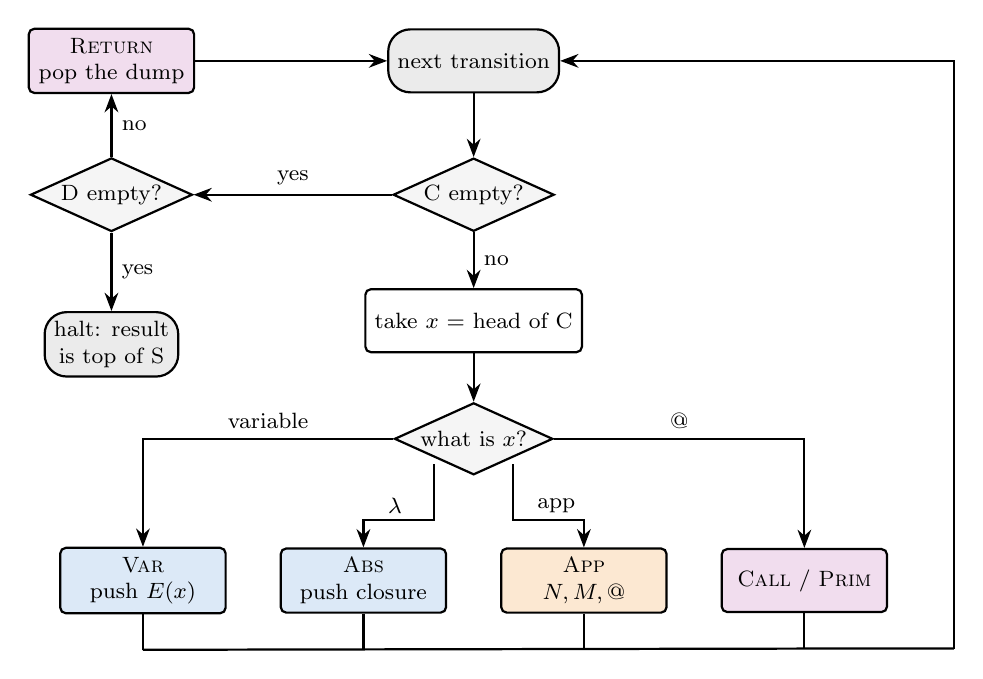
\begin{tikzpicture}[
  dec/.style={diamond, draw, thick, aspect=2.2, inner sep=1pt, fill=black!4, font=\footnotesize, align=center},
  box/.style={draw, thick, rounded corners=2pt, minimum width=2.1cm, minimum height=0.8cm, align=center, font=\footnotesize},
  term/.style={draw, thick, rounded corners=8pt, fill=black!8, align=center, font=\footnotesize, minimum height=0.8cm},
  line/.style={->, thick}]
\node[term] (top) at (0,1.7) {next transition};
\node[dec] (d1) at (0,0) {C empty?};
\node[dec] (d2) at (-4.6,0) {D empty?};
\node[term] (halt) at (-4.6,-1.9) {halt: result\\ is top of S};
\node[box, fill=dfill] (ret) at (-4.6,1.7) {\rul{Return}\\ pop the dump};
\node[box] (pop) at (0,-1.6) {take $x$ = head of C};
\node[dec] (d3) at (0,-3.1) {what is $x$?};
\node[box, fill=sfill] (var) at (-4.2,-4.9) {\rul{Var}\\ push $E(x)$};
\node[box, fill=sfill] (abs) at (-1.4,-4.9) {\rul{Abs}\\ push closure};
\node[box, fill=cfill] (app) at (1.4,-4.9) {\rul{App}\\ $N, M, \ap$};
\node[box, fill=dfill] (cal) at (4.2,-4.9) {\rul{Call} / \rul{Prim}};
\draw[line] (top) -- (d1);
\draw[line] (d1) -- node[above, font=\footnotesize] {yes} (d2);
\draw[line] (d2) -- node[right, font=\footnotesize] {yes} (halt);
\draw[line] (d2) -- node[right, font=\footnotesize] {no} (ret);
\draw[line] (ret) -- (top);
\draw[line] (d1) -- node[right, font=\footnotesize] {no} (pop);
\draw[line] (pop) -- (d3);
\draw[line] (d3.west) -| node[above, pos=0.25, font=\footnotesize] {variable} (var.north);
\draw[line] (d3.south) ++(-0.5,0.15) |- ($(abs.north)+(0,0.35)$) -- (abs.north);
\node[font=\footnotesize] at (-1.0,-3.95) {$\lambda$};
\draw[line] (d3.south) ++(0.5,0.15) |- ($(app.north)+(0,0.35)$) -- (app.north);
\node[font=\footnotesize] at (1.05,-3.95) {app};
\draw[line] (d3.east) -| node[above, pos=0.25, font=\footnotesize] {$\ap$} (cal.north);
\foreach \n in {var,abs,app,cal} {\draw[thick] (\n.south) -- ++(0,-0.45);}
\draw[thick] ($(var.south)+(0,-0.45)$) -- ($(cal.south)+(0,-0.45)$) -- ++(1.9,0) coordinate (cr);
\draw[line] (cr) |- (top.east);
\end{tikzpicture}
\caption{The machine as an interpreter loop. Every transition does a bounded
amount of work, apart from the environment lookup in \rul{Var}, which searches
a list.}
\label{fig:loop}
\end{figure}

% =====================================================================
\section{Worked examples}\label{sec:examples}

Throughout, $E_0 = [x\mapsto 4,\ y\mapsto 3]$. In the traces, each row
shows the state \emph{after} the rule named in the second column. Dump frames
are written $(S,E,C)$.

\subsection{The identity function}

Let $I = \lambda x.x$ and evaluate $I\,y$:

\begin{center}
\small
\begin{tabular}{>{$}r<{$} l >{$}l<{$} >{$}l<{$} >{$}l<{$} >{$}l<{$}}
\toprule
\# & rule & S & E & C & D\\
\midrule
0 & start & \emp & E_0 & [I\,y] & \emp\\
1 & \rul{App} & \emp & E_0 & [y,\ I,\ \ap] & \emp\\
2 & \rul{Var} & [3] & E_0 & [I,\ \ap] & \emp\\
3 & \rul{Abs} & [\cl{I}{E_0},\ 3] & E_0 & [\ap] & \emp\\
4 & \rul{Call} & \emp & [x\mapsto 3]\cdot E_0 & [x] & [(\emp, E_0, \emp)]\\
5 & \rul{Var} & [3] & [x\mapsto 3]\cdot E_0 & \emp & [(\emp, E_0, \emp)]\\
6 & \rul{Return} & [3] & E_0 & \emp & \emp\\
\bottomrule
\end{tabular}
\end{center}

Here $[x\mapsto 3]\cdot E_0$ is $E_0$ extended with $x\mapsto 3$. In step 4
the new binding of $x$ shadows the outer $x\mapsto 4$, so step 5 finds $3$.
The machine halts after step 6 with result $3$. Even the identity function
costs a dump frame: the call in step 4 saves a frame even though nothing remains to
be done after the call returns. \Cref{sec:compiling} returns to this point
under the heading of tail calls.

\subsection{Two arguments: \texorpdfstring{$K\,x\,y$}{K x y}}

Now the running example $K\,x\,y$ with $K = \lambda a.\lambda b.a$. Recall
that this means $(K\,x)\,y$. We abbreviate
$E_1 = [a\mapsto 4]\cdot E_0$, $E_2 = [b\mapsto 3]\cdot E_1$,
$\kappa_1 = \cl{K}{E_0}$ and $\kappa_2 = \cl{\lambda b.a}{E_1}$.

\begin{center}
\small
\begin{tabular}{>{$}r<{$} l >{$}l<{$} >{$}l<{$} >{$}l<{$} >{$}l<{$}}
\toprule
\# & rule & S & E & C & D\\
\midrule
0 & start & \emp & E_0 & [K\,x\,y] & \emp\\
1 & \rul{App} & \emp & E_0 & [y,\ K\,x,\ \ap] & \emp\\
2 & \rul{Var} & [3] & E_0 & [K\,x,\ \ap] & \emp\\
3 & \rul{App} & [3] & E_0 & [x,\ K,\ \ap,\ \ap] & \emp\\
4 & \rul{Var} & [4,\ 3] & E_0 & [K,\ \ap,\ \ap] & \emp\\
5 & \rul{Abs} & [\kappa_1,\ 4,\ 3] & E_0 & [\ap,\ \ap] & \emp\\
6 & \rul{Call} & \emp & E_1 & [\lambda b.a] & [([3], E_0, [\ap])]\\
7 & \rul{Abs} & [\kappa_2] & E_1 & \emp & [([3], E_0, [\ap])]\\
8 & \rul{Return} & [\kappa_2,\ 3] & E_0 & [\ap] & \emp\\
9 & \rul{Call} & \emp & E_2 & [a] & [(\emp, E_0, \emp)]\\
10 & \rul{Var} & [4] & E_2 & \emp & [(\emp, E_0, \emp)]\\
11 & \rul{Return} & [4] & E_0 & \emp & \emp\\
\bottomrule
\end{tabular}
\end{center}

A few things to notice:
\begin{itemize}
\item \textbf{The two $\ap$ markers.} Step 3 splits the inner application and
  puts a second $\ap$ in front of the first. The inner call is made first
  (step 6). The outer $\ap$ is saved on the dump with the stack $[3]$ and
  comes back into play only after the inner call returns (step 8).
\item \textbf{A function returned as a result.} The inner call returns a
  closure, $\kappa_2$, rather than a number. Its environment $E_1$ records
  that $a = 4$. When the frame from step 6 is popped in step 8, the binding
  $a\mapsto 4$ disappears from the machine's E register but survives inside
  $\kappa_2$. This is exactly why environments cannot be freed when a
  call returns, as they would be on a conventional stack.
\item \textbf{Comparison with substitution.} The closure $\kappa_2$ in step 8
  is the machine's representation of $\lambda b.4$, the intermediate term in
  \eqref{eq:ksub}. The two $\beta$-steps of \eqref{eq:ksub} are the two
  \rul{Call} transitions (steps 6 and 9). Everything else is bookkeeping that
  substitution hides.
\end{itemize}

\Cref{fig:heap} shows the machine's memory just after step 7. Nothing in the
machine is ever overwritten: $E_1$ extends $E_0$ by pointing at it, and the dump
frame points at the same $E_0$ that the closure's environment chain ends in.

\begin{figure}[t]
\centering
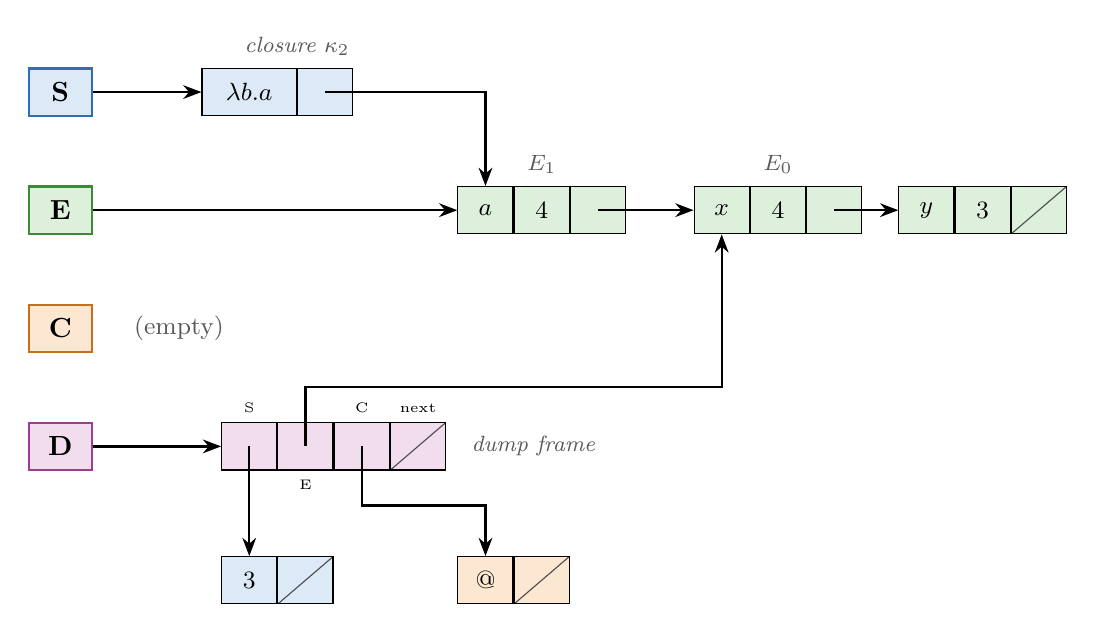
\begin{tikzpicture}[
  reg/.style={draw, thick, minimum width=0.8cm, minimum height=0.6cm, font=\bfseries},
  part/.style={cellb},
  nil/.style={cellb, path picture={\draw[black!70] (path picture bounding box.south west) -- (path picture bounding box.north east);}},
  dotp/.style={cellb, path picture={\fill (path picture bounding box.center) circle (1.6pt);}},
  lbl/.style={font=\footnotesize\itshape, text=black!65}]
\node[reg, fill=sfill, draw=sline] (S) at (0,0) {S};
\node[reg, fill=efill, draw=eline] (E) at (0,-1.5) {E};
\node[reg, fill=cfill, draw=cline] (C) at (0,-3.0) {C};
\node[reg, fill=dfill, draw=dline] (D) at (0,-4.5) {D};
% closure kappa2
\node[part, minimum width=1.2cm, fill=sfill] (kc) at (2.4,0) {$\lambda b.a$};
\node[dotp, right=0pt of kc, fill=sfill] (ke) {};
\node[lbl, above=1pt of kc.north east] {closure $\kappa_2$};
% E1
\node[part, fill=efill] (e1n) at (5.4,-1.5) {$a$};
\node[part, right=0pt of e1n, fill=efill] (e1v) {$4$};
\node[dotp, right=0pt of e1v, fill=efill] (e1p) {};
\node[lbl, above=1pt of e1v] {$E_1$};
% E0
\node[part, fill=efill] (e0n) at (8.4,-1.5) {$x$};
\node[part, right=0pt of e0n, fill=efill] (e0v) {$4$};
\node[dotp, right=0pt of e0v, fill=efill] (e0p) {};
\node[lbl, above=1pt of e0v] {$E_0$};
\node[part, fill=efill] (e0bn) at (11.0,-1.5) {$y$};
\node[part, right=0pt of e0bn, fill=efill] (e0bv) {$3$};
\node[nil, right=0pt of e0bv, fill=efill] (e0bp) {};
% stack element pointer from S
\draw[ptr] (S) -- (kc);
\draw[ptr] (ke.center) -| (e1n.north);
\draw[ptr] (E) -- (e1n);
\draw[ptr] (e1p.center) -- (e0n);
\draw[ptr] (e0p.center) -- (e0bn);
\node[right=4mm of C, text=black!65] (cempty) {(empty)};
% dump frame
\node[dotp, fill=dfill] (fS) at (2.4,-4.5) {};
\node[dotp, right=0pt of fS, fill=dfill] (fE) {};
\node[dotp, right=0pt of fE, fill=dfill] (fC) {};
\node[nil, right=0pt of fC, fill=dfill] (fD) {};
\node[lbl, right=2mm of fD] {dump frame};
\foreach \n/\t in {fS/S, fC/C, fD/next} {\node[font=\tiny, above=0pt of \n] {\t};}
\node[font=\tiny, below=0pt of fE] {E};
\draw[ptr] (D) -- (fS);
\node[part, fill=sfill] (v3) at (2.4,-6.2) {$3$};
\node[nil, right=0pt of v3, fill=sfill] (v3p) {};
\draw[ptr] (fS.center) -- ++(0,-0.6) -| (v3.north);
\node[part, fill=cfill] (at) at (5.4,-6.2) {$\ap$};
\node[nil, right=0pt of at, fill=cfill] (atp) {};
\draw[ptr] (fC.center) -- ++(0,-0.75) -| (at.north);
\draw[ptr] (fE.center) -- ++(0,0.75) -| (e0n.south);
\end{tikzpicture}
\caption{The machine's memory after step 7 of the $K\,x\,y$ trace. Cells with a
dot hold a pointer, and a slash marks the end of a list. The stack holds one
closure whose environment is $E_1$. The dump frame remembers the outer
computation: stack $[3]$, environment $E_0$, and control $[\ap]$. The
environments form linked lists with a shared tail.}
\label{fig:heap}
\end{figure}

\subsection{Lexical scope in action}

Finally, the term $T$ from \eqref{eq:lexical}. Its trace takes 16 steps, and we
summarise the important moments rather than listing all of them:
\begin{enumerate}[nosep]
\item The argument $\lambda z.x$ is evaluated first, by \rul{Abs} in $E_0$,
  giving $\kappa = \cl{\lambda z.x}{E_0}$.
\item The outer call binds $f\mapsto\kappa$, producing $E_f = [f\mapsto\kappa]\cdot E_0$.
\item The inner call $(\lambda x.f\,x)\,y$ binds $x\mapsto 3$, producing
  $E_x = [x\mapsto 3]\cdot E_f$.
\item Evaluating $f\,x$ in $E_x$ pushes $3$ and $\kappa$, and \rul{Call} runs
  the body $x$ of $\kappa$ in $[z\mapsto 3]\cdot E_0$, \emph{not} in $E_x$.
\item \rul{Var} finds $x\mapsto 4$. The result is $4$, as substitution
  predicted.
\end{enumerate}
\Cref{fig:lexical} shows this picture. The dump reaches depth $3$ at
step 4: the outer call, the inner call and the call of $\kappa$ are all
pending at once.

% =====================================================================
\section{What the machine computes}\label{sec:meaning}

\subsection{Values and read-back}

The machine's results are machine values. For a constant, that is all there is to
say. A closure, however, is not a $\lambda$-term, so to compare the machine
with the $\lambda$-calculus we need to turn closures back into terms. Plotkin
called this function $\Real$~\cite{plotkin75}:
\[
  \Real(c) = c \quad\text{for constants,}\qquad
  \Real(\cl{\lambda x.B}{E}) = (\lambda x.B)\bigl[\Real(E(y_1))/y_1, \dots, \Real(E(y_k))/y_k\bigr],
\]
where $y_1,\dots,y_k$ are the free variables of $\lambda x.B$. In words: take the
code and substitute in whatever its environment says about its free variables.
For instance, $\Real(\kappa_2) = \Real(\cl{\lambda b.a}{[a\mapsto 4]\cdot E_0}) = \lambda b.4$.

\begin{theorem}[Correctness, informally]
Let $M$ be a term whose free variables are bound to constants by $E_0$.
Starting from $\st{\emp}{E_0}{[M]}{\emp}$, the machine halts with value
$v$ on top of the stack if and only if $M$ reduces under call-by-value to a
value $V$, and in that case $\Real(v) = V$. If $M$ has no call-by-value
value, the machine runs forever or gets stuck.
\end{theorem}

Plotkin proved a theorem of this form for Landin's machine in 1975, in the same
paper that defined the call-by-value $\lambda$-calculus~\cite{plotkin75}.
To see why such a theorem holds, read each machine state back as a
$\lambda$-term, using $\Real$ on the values and plugging the result into the
computations saved on the dump. Then check that every transition either leaves
that term unchanged (bookkeeping) or performs one $\beta_v$-step.

\subsection{Consequences}

\begin{itemize}
\item \textbf{The machine stops at WHNF.} If $M$ evaluates to a function, the
  result is a closure whose body has \emph{not} been evaluated. In
  \cref{sec:programming} this means that the closure returned by
  ``factorial of 3'' does not yet contain the number 6. It is a recipe that
  will produce 6 when used.
\item \textbf{Evaluation order is fixed but rarely visible.} Arguments are
  evaluated right to left. For terms without side effects, the order only
  matters when two subterms fail differently: if both $M$ and $N$ diverge or
  get stuck, it determines which failure you see first.
\item \textbf{Stuck states are possible.} The pure rules have no answer for
  an unbound variable, or for $\ap$ with a constant such as $4$ in function
  position. The C program aborts in the first case, and in the second it
  silently consumes the $\ap$ and leaves both values on the stack
  (\cref{ex:stuck}).
\end{itemize}

% =====================================================================
\section{Programming the machine}\label{sec:programming}

With only $\lambda$, variables and application, data has to be encoded as
functions. This section uses the standard Church encodings and runs into two
interesting obstacles, both caused by call-by-value.

\subsection{Booleans and numbers}

\begin{align*}
  \mathit{true} &= \lambda x.\lambda y.x &
  \mathit{false} &= \lambda x.\lambda y.y\\
  \underline{0} &= \lambda f.\lambda x.x &
  \underline{1} &= \lambda f.\lambda x.f\,x\\
  \mathit{succ} &= \lambda n.\lambda f.\lambda x.\,f\,(n\,f\,x) &
  \mathit{times} &= \lambda m.\lambda n.\lambda f.\,m\,(n\,f)\\
  \mathit{iszero} &= \lambda n.\,n\,(\lambda x.\mathit{false})\,\mathit{true} &
  \mathit{pred} &= \lambda n.\lambda f.\lambda x.\,n\,(\lambda g.\lambda h.\,h\,(g\,f))\,(\lambda u.x)\,(\lambda u.u)
\end{align*}
The numeral $\underline{n}$ applies its first argument $n$ times. A boolean
selects one of its two arguments, so ``if $b$ then $P$ else $Q$'' is
written $b\,P\,Q$. The predecessor function is the well-known tricky one: it
rebuilds the numeral one step behind, using the pair-like functions
$\lambda g.\lambda h.h\,(g\,f)$.

The companion program checks results by asking yes/no questions, since
booleans are easy to recognise on the stack: the machine value of
$\mathit{true}$ prints as the closure $\cl{\lambda y.x}{\dots}$ and
$\mathit{false}$ as $\cl{\lambda y.y}{\dots}$.

\subsection{Obstacle 1: a strict \emph{if}}

Under call-by-value, $b\,P\,Q$ evaluates \emph{both} $P$ and $Q$ before $b$
gets to choose. That is wasteful at best. When one branch is a recursive
call, it never terminates, because the recursion is unfolded whether or not
it is needed.

The standard fix is to \emph{delay} each branch by wrapping it in a
$\lambda$, which the machine will not evaluate inside (rule \rul{Abs}). Then
the selected branch is called with a dummy argument:
\[
  \text{if } b \text{ then } P \text{ else } Q
  \quad\leadsto\quad
  b\;(\lambda d.P)\;(\lambda d.Q)\;\mathit{dummy}.
\]
A function used this way, purely to postpone evaluation, is called a
\emph{thunk}.

\subsection{Obstacle 2: recursion without \texorpdfstring{$Y$}{Y}}

The usual fixed-point combinator
$Y = \lambda f.(\lambda x.f\,(x\,x))\,(\lambda x.f\,(x\,x))$ is useless under
call-by-value. To evaluate $Y\,H$ the machine must evaluate the argument
$x\,x$ before calling $f$, and $x\,x$ unfolds into $H\,(x\,x)$, whose argument
must again be evaluated first, and so on forever. The fix is the same trick
as before, delaying with a $\lambda$. Eta-expanding $x\,x$ to $\lambda y.x\,x\,y$
gives the call-by-value fixed-point combinator
\[
  Z = \lambda f.\,(\lambda x.\,f\,(\lambda y.\,x\,x\,y))\,(\lambda x.\,f\,(\lambda y.\,x\,x\,y)).
\]
Now the argument passed to $f$ is a $\lambda$, which is already a value, and the
self-application happens only when the recursive function is actually called.

\subsection{Factorial}

Putting both fixes together:
\begin{align*}
  H &= \lambda f.\lambda n.\;\mathit{iszero}\,n\;(\lambda d.\underline{1})\;
      (\lambda d.\,\mathit{times}\,n\,(f\,(\mathit{pred}\,n)))\;n\\
  \mathit{fac} &= Z\,H
\end{align*}
The trailing $n$ is the dummy argument, and any value would do. The companion
program verifies $\mathit{fac}\,\underline{3} = \underline{6}$ without ever
printing a numeral: $\mathit{iszero}\,(\mathit{pred}^5\,(\mathit{fac}\,\underline{3}))$
evaluates to $\mathit{false}$ and
$\mathit{iszero}\,(\mathit{pred}^6\,(\mathit{fac}\,\underline{3}))$ to $\mathit{true}$.
Both checks are needed, because $\mathit{pred}\,\underline{0} = \underline{0}$ in
this encoding, so the second alone would also accept any number below 6.
\Cref{sec:primitives} shows a more direct way to read a numeral.

\subsection{What it costs}

\Cref{tab:fac} gives the number of transitions and the maximum dump depth for
evaluating $\mathit{fac}\,\underline{n}$ (to WHNF) on the companion program,
and \cref{fig:dump} shows the dump depth at every step of
$\mathit{fac}\,\underline{2}$.

\begin{table}[t]
\centering
\begin{tabular}{rrr}
\toprule
$n$ & transitions & max.\ dump depth\\
\midrule
0 & 51 & 3\\
1 & 151 & 8\\
2 & 341 & 13\\
3 & 626 & 18\\
4 & 1026 & 23\\
\bottomrule
\end{tabular}
\caption{Cost of evaluating $\mathit{fac}\,\underline{n}$ to weak head normal
form. The dump depth grows by exactly 5 per level of recursion. The
number of transitions grows faster than linearly (\cref{ex:quadratic}).}
\label{tab:fac}
\end{table}

\begin{figure}[t]
\centering
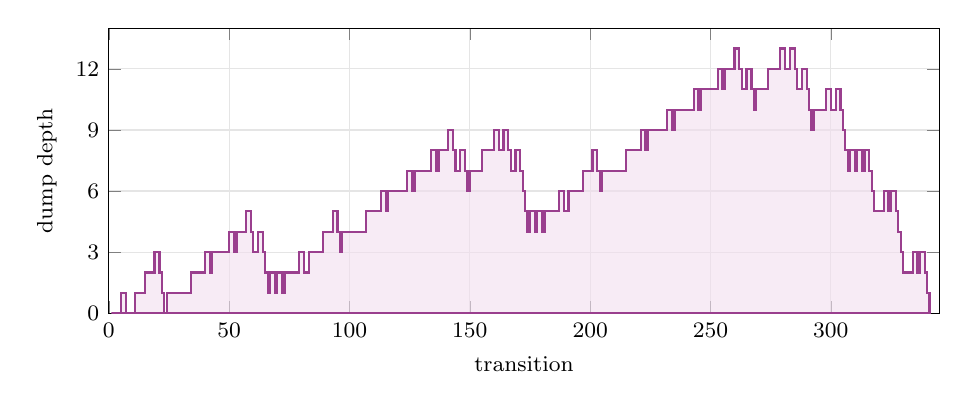
\begin{tikzpicture}
\begin{axis}[
  width=\linewidth, height=5.2cm,
  xlabel={transition}, ylabel={dump depth},
  xmin=0, xmax=345, ymin=0, ymax=14,
  ytick={0,3,6,9,12},
  grid=major, grid style={black!10},
  tick label style={font=\footnotesize}, label style={font=\footnotesize},
]
\addplot[const plot, dline, thick, fill=dfill, fill opacity=0.6] coordinates {
(1,0) (2,0) (3,0) (4,0) (5,1) (6,1) (7,0) (8,0) (9,0) (10,0) (11,1) (12,1) (13,1) (14,1) (15,2)
(16,2) (17,2) (18,2) (19,3) (20,3) (21,2) (22,1) (23,0) (24,1) (25,1) (26,1) (27,1) (28,1) (29,1)
(30,1) (31,1) (32,1) (33,1) (34,2) (35,2) (36,2) (37,2) (38,2) (39,2) (40,3) (41,3) (42,2) (43,3)
(44,3) (45,3) (46,3) (47,3) (48,3) (49,3) (50,4) (51,4) (52,3) (53,4) (54,4) (55,4) (56,4) (57,5)
(58,5) (59,4) (60,3) (61,3) (62,4) (63,4) (64,3) (65,2) (66,1) (67,2) (68,2) (69,1) (70,2) (71,2)
(72,1) (73,2) (74,2) (75,2) (76,2) (77,2) (78,2) (79,3) (80,3) (81,2) (82,2) (83,3) (84,3) (85,3)
(86,3) (87,3) (88,3) (89,4) (90,4) (91,4) (92,4) (93,5) (94,5) (95,4) (96,3) (97,4) (98,4) (99,4)
(100,4) (101,4) (102,4) (103,4) (104,4) (105,4) (106,4) (107,5) (108,5) (109,5) (110,5) (111,5)
(112,5) (113,6) (114,6) (115,5) (116,6) (117,6) (118,6) (119,6) (120,6) (121,6) (122,6) (123,6)
(124,7) (125,7) (126,6) (127,7) (128,7) (129,7) (130,7) (131,7) (132,7) (133,7) (134,8) (135,8)
(136,7) (137,8) (138,8) (139,8) (140,8) (141,9) (142,9) (143,8) (144,7) (145,7) (146,8) (147,8)
(148,7) (149,6) (150,7) (151,7) (152,7) (153,7) (154,7) (155,8) (156,8) (157,8) (158,8) (159,8)
(160,9) (161,9) (162,8) (163,8) (164,9) (165,9) (166,8) (167,7) (168,7) (169,8) (170,8) (171,7)
(172,6) (173,5) (174,4) (175,5) (176,5) (177,4) (178,5) (179,5) (180,4) (181,5) (182,5) (183,5)
(184,5) (185,5) (186,5) (187,6) (188,6) (189,5) (190,5) (191,6) (192,6) (193,6) (194,6) (195,6)
(196,6) (197,7) (198,7) (199,7) (200,7) (201,8) (202,8) (203,7) (204,6) (205,7) (206,7) (207,7)
(208,7) (209,7) (210,7) (211,7) (212,7) (213,7) (214,7) (215,8) (216,8) (217,8) (218,8) (219,8)
(220,8) (221,9) (222,9) (223,8) (224,9) (225,9) (226,9) (227,9) (228,9) (229,9) (230,9) (231,9)
(232,10) (233,10) (234,9) (235,10) (236,10) (237,10) (238,10) (239,10) (240,10) (241,10) (242,10)
(243,11) (244,11) (245,10) (246,11) (247,11) (248,11) (249,11) (250,11) (251,11) (252,11) (253,12)
(254,12) (255,11) (256,12) (257,12) (258,12) (259,12) (260,13) (261,13) (262,12) (263,11) (264,11)
(265,12) (266,12) (267,11) (268,10) (269,11) (270,11) (271,11) (272,11) (273,11) (274,12) (275,12)
(276,12) (277,12) (278,12) (279,13) (280,13) (281,12) (282,12) (283,13) (284,13) (285,12) (286,11)
(287,11) (288,12) (289,12) (290,11) (291,10) (292,9) (293,10) (294,10) (295,10) (296,10) (297,10)
(298,11) (299,11) (300,10) (301,10) (302,11) (303,11) (304,10) (305,9) (306,8) (307,7) (308,8)
(309,8) (310,7) (311,8) (312,8) (313,7) (314,8) (315,8) (316,7) (317,6) (318,5) (319,5) (320,5)
(321,5) (322,6) (323,6) (324,5) (325,6) (326,6) (327,5) (328,4) (329,3) (330,2) (331,2) (332,2)
(333,2) (334,3) (335,3) (336,2) (337,3) (338,3) (339,2) (340,1) (341,0)
} \closedcycle;
\end{axis}
\end{tikzpicture}
\caption{Dump depth during the 341 transitions of $\mathit{fac}\,\underline{2}$.
Each rise is a call and each fall a return. The depth climbs in two
stages, one per level of recursion: it peaks at 9 around transition 140,
falls back only partway, then climbs to 13 between transitions 260 and 285
before the whole computation unwinds. Frames from the outer level are still
pending while the inner level runs.}
\label{fig:dump}
\end{figure}

The dump grows because the frames below a recursive call are waiting for it
to finish. Some frames, however, belong to calls whose caller has nothing left
to do afterwards. The identity example in \cref{sec:examples} saves such a frame,
with an empty control. \rul{Return} into such a frame just returns again. A
machine that recognises these \emph{tail calls} and does not push a frame
for them uses less space (\cref{sec:tailcalls,ex:tail}).

% =====================================================================
\section{Primitives and constants}\label{sec:primitives}

Real programs need numbers and arithmetic. These are added as
\emph{primitive} values, together with a function $\delta$ that says what each
primitive does when applied. This is rule \rul{Prim}:
\[
  \st{f : v : S}{E}{\ap : C}{D} \trans \st{\delta(f,v) : S}{E}{C}{D}.
\]
No dump frame is needed: the primitive's work is done in a single step.

\paragraph{One argument.} $\delta(\mathit{SUCC}, n) = n+1$. With $\mathit{SUCC}$
available, a Church numeral can be converted to a machine integer by applying
it: $\underline{6}\;\mathit{SUCC}\;0$ evaluates to the constant $6$. This is the
easiest way to see the result of $\mathit{fac}\,\underline{3}$ (\cref{ex:prims}).

\paragraph{Curried primitives.} A two-argument operation such as addition
receives its arguments one at a time. One solution is to let $\delta$ return a
new primitive that remembers the first argument:
$\delta(\mathit{PLUS}, m) = \mathit{PLUS}_m$ and
$\delta(\mathit{PLUS}_m, n) = m+n$. This is a tiny closure in disguise.

\paragraph{Conditionals.} A primitive receives its arguments already
evaluated, so an $\mathit{IF}$ primitive would suffer from exactly the strictness
problem described above. Implementations therefore treat conditionals
specially. The compiled machine in \cref{sec:compiling} uses dedicated
instructions.

The companion C program reserves a value tag \texttt{PRIM} and an enumeration
of primitive operations (\texttt{PLUS}, \texttt{MINUS}, \texttt{IF}), but the
\rul{Prim} case of its main loop is still an empty stub.

% =====================================================================
\section{Inside an implementation}\label{sec:implementation}

This section reads the companion program \texttt{secd23.c}, about 400 lines of
C. It is deliberately small, and it is a good model of how the rules
become code, including one way to get it wrong.

\subsection{Representation}

Expressions, values and environment bindings are each a C struct. Each struct
has a \texttt{next} pointer, which lets it be threaded directly onto a list:
\begin{lstlisting}
typedef enum {ID, LAM, APP, AT} exptag;           /* AT is the @ marker */
typedef enum {INT, PRIM, CLOSURE} whnftag;

typedef struct exp_cell  { struct exp_cell  *next; exptag tag;  ... } *EXP;
typedef struct whnf_cell { struct whnf_cell *next; whnftag tag; ... } *WHNF;
typedef struct env_cell  { struct env_cell  *next; char name; WHNF value; } *ENV;

typedef struct state_cell {
  WHNF stack;                 /* S: list of values, linked by next   */
  ENV environment;            /* E: list of bindings, linked by next */
  EXP control;                /* C: list of expressions and @ marks  */
  struct state_cell *dump;    /* D: list of saved states             */
} *STATE;
\end{lstlisting}
The stack is a list of \texttt{WHNF} cells and the control is a list of
\texttt{EXP} cells, both linked through the cells' own \texttt{next} fields
rather than through separate list nodes. Lists linked this way are called
\emph{intrusive}. A dump frame is just another \texttt{STATE}, so the dump is
a list of states. Variable names are single characters.

\subsection{From rules to code}

The main loop of \cref{fig:loop} is a \texttt{while} over
\texttt{machine->control || machine->dump}. The correspondence is direct:

\begin{center}
\small
\begin{tabularx}{\linewidth}{@{}l X@{}}
\toprule
rule & code\\
\midrule
\rul{Var} & \texttt{push(valueof(x->expkind.id, machine->environment), machine)}. \texttt{valueof} searches the environment list and aborts when the name is unbound.\\
\rul{Abs} & \texttt{push(mkclosure(body, bv, machine->environment), machine)}.\\
\rul{App} & Build the control cells $N$, $M$, $\ap$ and link them in front of the rest of the control (excerpt below).\\
\rul{Call} & Allocate a \texttt{STATE} holding the stack below the argument, plus the current environment and control, and push it on the dump. Bind the parameter in front of the closure's environment and start the body.\\
\rul{Return} & Link the top of the stack in front of the saved stack, then restore the environment, control and dump from the frame.\\
\bottomrule
\end{tabularx}
\end{center}

Here is the \rul{App} case, with its debugging output removed:
\begin{lstlisting}
} else if (x->tag == APP) {                     /* case 1c */
  F = copyexp(x->expkind.app.rator);
  A = copyexp(x->expkind.app.rand);
  e = mkat();                                   /* the @ marker */
  e->next = machine->control;
  F->next = e;
  A->next = F;
  machine->control = A;                         /* C := A : F : @ : C */
}
\end{lstlisting}
The calls to \texttt{copyexp} are the important detail. The next section
explains why they are there.

\subsection{A lesson in sharing}\label{sec:sharing}

The original version of the program, \texttt{secd.c}, had the same code without
the copies: it set \texttt{F->next} and \texttt{A->next} on the subterms of the
program itself. The program built its terms in C by reusing named pieces such as
$\mathit{succ}$ in several places, so the term was not a tree but a DAG with
shared nodes. That works for read-only data, but the \texttt{next} field is not
read-only.

Consider $\mathit{succ}\,(\mathit{succ}\,\underline{0})$, where both occurrences
of $\mathit{succ}$ are the \emph{same} node. The first \rul{App} sets
$\mathit{succ}.\texttt{next} = \ap_1$. The second sets
$\mathit{succ}.\texttt{next} = \ap_2$, overwriting the first, and
$\ap_2.\texttt{next}$ is the old rest of the control, which begins with
$\mathit{succ}$ itself. The control list now contains a cycle
(\cref{fig:cycle}), and the machine applies $\mathit{succ}$ over and over
until it crashes. In the original program this happened within a few steps.

\begin{figure}[t]
\centering
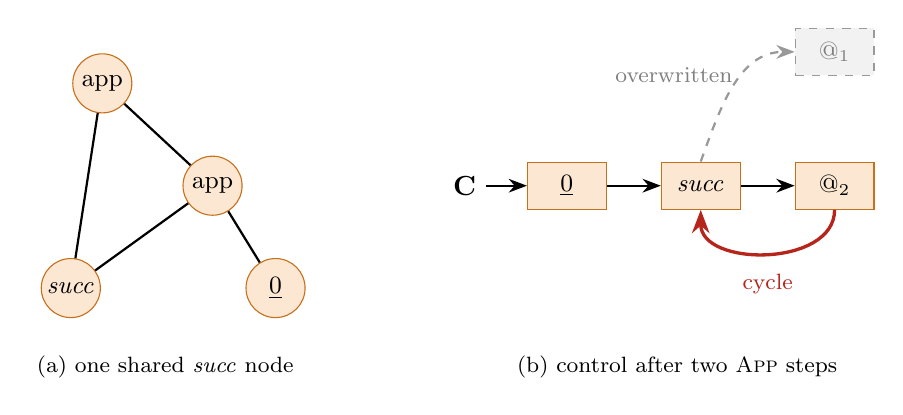
\begin{tikzpicture}[
  tn/.style={draw=cline, fill=cfill, circle, inner sep=1.5pt, minimum size=0.75cm},
  ccell/.style={draw=cline, fill=cfill, minimum width=1.0cm, minimum height=0.6cm},
  lost/.style={draw=black!40, dashed, fill=black!5, text=black!50, minimum width=1.0cm, minimum height=0.6cm}]
% DAG
\node[tn] (a1) at (0,0) {app};
\node[tn] (a2) at (1.4,-1.3) {app};
\node[tn] (s) at (-0.4,-2.6) {$\mathit{succ}$};
\node[tn] (z) at (2.2,-2.6) {$\underline{0}$};
\draw[thick] (a1) -- (s); \draw[thick] (a1) -- (a2);
\draw[thick] (a2) -- (s); \draw[thick] (a2) -- (z);
\node[font=\footnotesize] at (0.8,-3.6) {(a) one shared $\mathit{succ}$ node};
% control list
\node[font=\bfseries] (Cr) at (4.6,-1.3) {C};
\node[ccell] (cz) at (5.9,-1.3) {$\underline{0}$};
\node[ccell] (cs) at (7.6,-1.3) {$\mathit{succ}$};
\node[ccell] (c2) at (9.3,-1.3) {$\ap_2$};
\node[lost] (c1) at (9.3,0.4) {$\ap_1$};
\draw[ptr] (Cr) -- (cz);
\draw[ptr] (cz) -- (cs);
\draw[ptr] (cs) -- (c2);
\draw[ptr, BrickRed, very thick] (c2.south) to[out=-90, in=-90, looseness=1.1] (cs.south);
\draw[->, thick, dashed, black!40] (cs.north) to[out=70, in=180] node[left, font=\footnotesize, text=black!50, pos=0.6] {overwritten} (c1.west);
\node[font=\footnotesize, BrickRed] at (8.45,-2.55) {cycle};
\node[font=\footnotesize] at (7.3,-3.6) {(b) control after two \rul{App} steps};
\end{tikzpicture}
\caption{How sharing broke the original program. (a) The term
$\mathit{succ}\,(\mathit{succ}\,\underline{0})$ built with a single $\mathit{succ}$ node.
(b) Each \rul{App} step writes the \texttt{next} field of the node it puts on the
control. The second write overwrites the first, and the control list loops
back on itself.}
\label{fig:cycle}
\end{figure}

The fix is to never write \texttt{next} on a cell that might be shared. The
program copies an expression cell (a shallow copy: only the cell, not its
subterms) before linking it into the control, and copies a value cell before
pushing it. Values stored in environments are copies too. Otherwise a value
that sat on the stack would drag the rest of the stack along with it through
its \texttt{next} field.

The lesson goes beyond this program. The abstract machine is purely
functional: no rule ever modifies an existing structure. An implementation
that saves memory by updating cells in place must make sure that no other
part of the state can see those cells.

\subsection{Memory}

The program never frees anything. A real implementation needs a garbage
collector, and the $K\,x\,y$ example shows why a stack discipline is not
enough: the environment $E_1$ outlives the call that created it, because
$\kappa_2$ still points to it. Environments therefore live in the heap and
are shared, and the structure of linked environments is sometimes called a
\emph{spaghetti stack}. SECD machines have always assumed a Lisp-style heap
with garbage collection.

% =====================================================================
\section{Compiling for the SECD machine}\label{sec:compiling}

Look again at rule \rul{App}. Each time an application reaches the front of
the control, the machine re-derives the same postfix sequence $N, M, \ap$. It
does this every time the code runs. Inside a loop or a recursive function,
the same term is taken apart again and again. Since the sequence depends
only on the term, not on any run-time value, it can be computed once, in
advance. That is compilation.

\subsection{Instructions}

The compiled SECD machine, in the style of Henderson~\cite{henderson80},
replaces the control's $\lambda$-terms by \emph{instructions}. Variables
are replaced by \emph{de Bruijn indices}~\cite{debruijn72}: the variable's
position in the environment, counting from the front. This works because the
shape of the environment at each point in the program is known statically.
It is the list of enclosing binders. Lookup by name becomes lookup by
position.

\begin{center}
\small
\begin{tabular}{@{}l l@{\;}c@{\;}l@{}}
\toprule
instruction & \multicolumn{3}{l}{transition}\\
\midrule
\ins{LD} $i$ & $\st{S}{E}{\ins{LD}\,i : C}{D}$ &$\to$& $\st{E(i) : S}{E}{C}{D}$\\
\ins{LDC} $k$ & $\st{S}{E}{\ins{LDC}\,k : C}{D}$ &$\to$& $\st{k : S}{E}{C}{D}$\\
\ins{LDF} $c$ & $\st{S}{E}{\ins{LDF}\,c : C}{D}$ &$\to$& $\st{\cl{c}{E} : S}{E}{C}{D}$\\
\ins{AP} & $\st{\cl{c}{E'} : v : S}{E}{\ins{AP} : C}{D}$ &$\to$& $\st{\emp}{v : E'}{c}{(S,E,C) : D}$\\
\ins{RTN} & $\st{v : S}{E}{\ins{RTN} : C}{(S',E',C') : D}$ &$\to$& $\st{v : S'}{E'}{C'}{D}$\\
\bottomrule
\end{tabular}
\end{center}

A closure now pairs \emph{code} $c$, an instruction list, with an environment.
\ins{AP} is the old \rul{Call}, and \ins{RTN} is the old \rul{Return}, now
triggered by an explicit instruction instead of an empty control.

\subsection{The compiler}

The compiler $\mathcal{C}\sem{M}\rho$ takes a term and a \emph{compile-time
environment} $\rho$, the list of variable names that the run-time
environment will hold. It is three lines long, one per syntactic form:
\begin{align*}
  \mathcal{C}\sem{x}\rho &= [\ins{LD}\ i] \quad\text{where $i$ is the position of $x$ in $\rho$}\\
  \mathcal{C}\sem{\lambda x.M}\rho &= [\ins{LDF}\ (\mathcal{C}\sem{M}(x : \rho) \mathbin{+\!\!+} [\ins{RTN}])]\\
  \mathcal{C}\sem{M\,N}\rho &= \mathcal{C}\sem{N}\rho \mathbin{+\!\!+} \mathcal{C}\sem{M}\rho \mathbin{+\!\!+} [\ins{AP}]
\end{align*}
The third line is exactly rule \rul{App}, applied once, at compile time, to
every application in the program.

For $K\,x\,y$ with $\rho_0 = [x, y]$, so $x$ is index 0 and $y$ index 1:
\[
  \mathcal{C}\sem{K\,x\,y}\rho_0 =
  [\ins{LD}\ 1,\ \ins{LD}\ 0,\ \ins{LDF}\ c_1,\ \ins{AP},\ \ins{AP}]
  \quad\text{where}\quad
  c_1 = [\ins{LDF}\ c_2,\ \ins{RTN}],\quad
  c_2 = [\ins{LD}\ 1,\ \ins{RTN}].
\]
In $c_2$, the body of $\lambda b.a$, the compile-time environment is
$[b, a, x, y]$, so $a$ is index 1. \Cref{fig:code} draws the code, which is
a set of instruction lists linked by the pointers inside \ins{LDF}.

\begin{figure}[t]
\centering
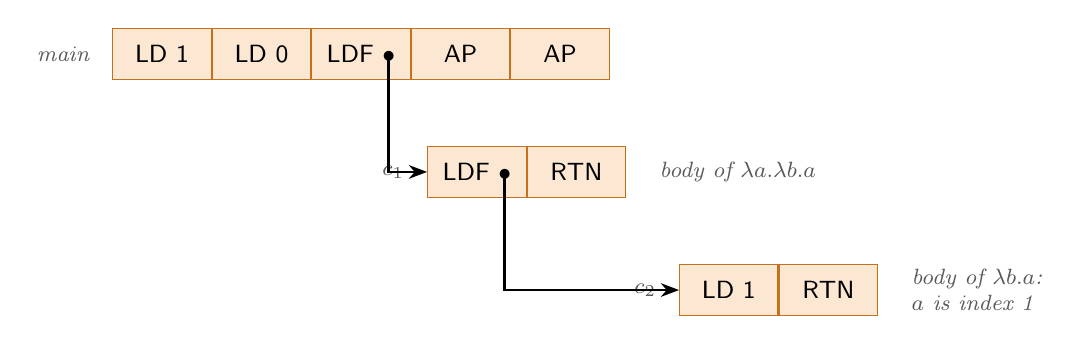
\begin{tikzpicture}[
  ic/.style={draw=cline, fill=cfill, minimum height=0.65cm, minimum width=1.25cm, font=\small\sffamily},
  lbl/.style={font=\footnotesize\itshape, text=black!65}]
\node[lbl, anchor=east] at (-0.8,0) {main};
\node[ic] (m1) at (0,0) {LD 1};
\node[ic, right=0pt of m1] (m2) {LD 0};
\node[ic, right=0pt of m2] (m3) {LDF $\bullet$};
\node[ic, right=0pt of m3] (m4) {AP};
\node[ic, right=0pt of m4] (m5) {AP};
\node[lbl, anchor=east] at (3.2,-1.5) {$c_1$};
\node[ic] (a1) at (4.0,-1.5) {LDF $\bullet$};
\node[ic, right=0pt of a1] (a2) {RTN};
\node[lbl, anchor=east] at (6.4,-3.0) {$c_2$};
\node[ic] (b1) at (7.2,-3.0) {LD 1};
\node[ic, right=0pt of b1] (b2) {RTN};
\draw[ptr] ($(m3.center)+(0.35,0)$) |- (a1.west);
\draw[ptr] ($(a1.center)+(0.35,0)$) |- (b1.west);
\node[lbl, align=left, right=3mm of b2] {body of $\lambda b.a$:\\ $a$ is index 1};
\node[lbl, align=left, right=3mm of a2] {body of $\lambda a.\lambda b.a$};
\end{tikzpicture}
\caption{Compiled code for $K\,x\,y$. Each $\lambda$ becomes a separate
instruction list, referenced by the \ins{LDF} that creates its closures. The
code is never modified at run time, so it can be shared freely.}
\label{fig:code}
\end{figure}

Running it with run-time environment $[4, 3]$:
\begin{center}
\small
\begin{tabular}{>{$}r<{$} l >{$}l<{$} >{$}l<{$} >{$}l<{$} >{$}l<{$}}
\toprule
\# & instr. & S & E & C & D\\
\midrule
0 & start & \emp & [4,3] & [\ins{LD}\,1, \ins{LD}\,0, \ins{LDF}\,c_1, \ins{AP}, \ins{AP}] & \emp\\
1 & \ins{LD} 1 & [3] & [4,3] & [\ins{LD}\,0, \ins{LDF}\,c_1, \ins{AP}, \ins{AP}] & \emp\\
2 & \ins{LD} 0 & [4,3] & [4,3] & [\ins{LDF}\,c_1, \ins{AP}, \ins{AP}] & \emp\\
3 & \ins{LDF} & [\cl{c_1}{[4,3]}, 4, 3] & [4,3] & [\ins{AP}, \ins{AP}] & \emp\\
4 & \ins{AP} & \emp & [4,4,3] & c_1 & [([3], [4,3], [\ins{AP}])]\\
5 & \ins{LDF} & [\cl{c_2}{[4,4,3]}] & [4,4,3] & [\ins{RTN}] & [([3], [4,3], [\ins{AP}])]\\
6 & \ins{RTN} & [\cl{c_2}{[4,4,3]}, 3] & [4,3] & [\ins{AP}] & \emp\\
7 & \ins{AP} & \emp & [3,4,4,3] & c_2 & [(\emp, [4,3], \emp)]\\
8 & \ins{LD} 1 & [4] & [3,4,4,3] & [\ins{RTN}] & [(\emp, [4,3], \emp)]\\
9 & \ins{RTN} & [4] & [4,3] & \emp & \emp\\
\bottomrule
\end{tabular}
\end{center}
Compare this with the interpreted trace in \cref{sec:examples}: the same calls and returns
happen at the same moments, but the two \rul{App} steps are gone (9
transitions instead of 11), and every variable lookup is an index rather
than a search by name. Notice also that the sharing bug of
\cref{sec:sharing} cannot arise here. The control is a pointer into
immutable code, and advancing it never writes anything.

\subsection{Conditionals}

With primitive booleans, a conditional compiles to two code blocks and a
selection instruction. The dump saves the place to continue at afterwards:
\[
\begin{array}{@{}l@{\quad}r@{\;}c@{\;}l@{}}
\ins{SEL} & \st{b : S}{E}{\ins{SEL}\,c_t\,c_f : C}{D} &\to& \st{S}{E}{c_b}{C : D}\\
\ins{JOIN} & \st{S}{E}{[\ins{JOIN}]}{C : D} &\to& \st{S}{E}{C}{D}
\end{array}
\]
where $c_b$ is $c_t$ or $c_f$ depending on $b$, and both branches end in
\ins{JOIN}. Only the selected branch is ever executed, so the thunks of
\cref{sec:programming} are no longer needed.

\subsection{Tail calls}\label{sec:tailcalls}

An application whose result is immediately returned, compiled as
$\dots, \ins{AP}, \ins{RTN}$, pushes a dump frame only for \ins{RTN} to pop it
straight away. A \emph{tail-call} instruction avoids this by not saving a frame at all:
\[
  \ins{TAP}:\quad \st{\cl{c}{E'} : v : S}{E}{[\ins{TAP}]}{D} \;\to\; \st{\emp}{v : E'}{c}{D}.
\]
When the body of $c$ finishes, it returns directly to the caller's caller.
With \ins{TAP}, a loop written as tail recursion runs in constant dump
space. Scheme makes this behaviour mandatory, and it is the reason the
Scheme standard talks about ``proper tail recursion''.

% =====================================================================
\section{Relatives and descendants}\label{sec:relatives}

The SECD machine is the ancestor of a family of abstract machines. Each one
changes one of its design decisions (\cref{fig:family}).

\begin{figure}[t]
\centering
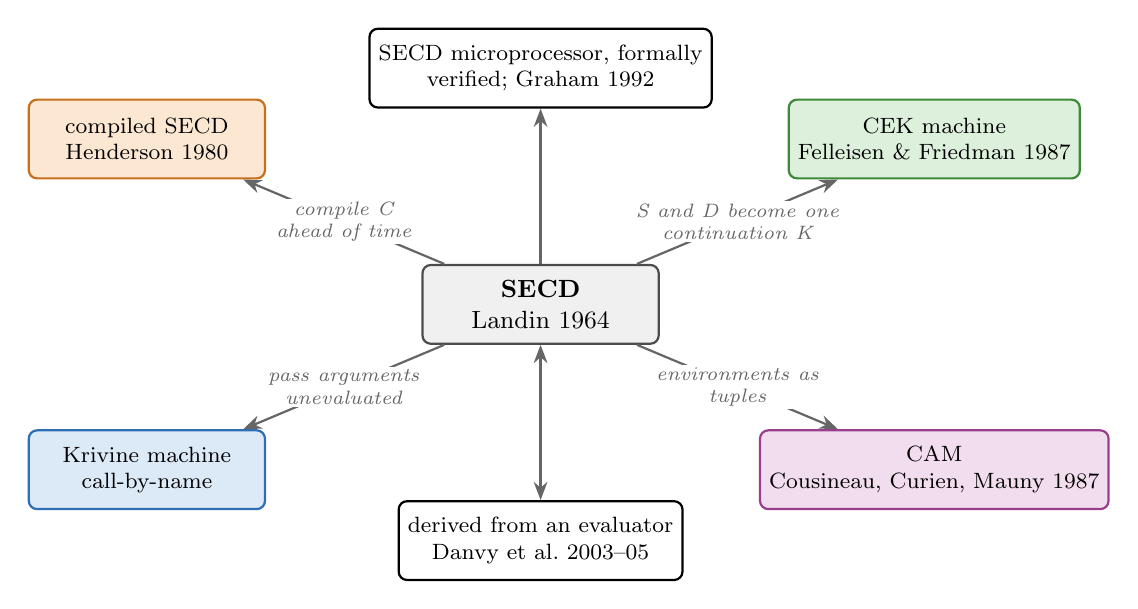
\begin{tikzpicture}[
  m/.style={draw, thick, rounded corners=3pt, align=center, fill=white, minimum width=3.0cm, minimum height=1.0cm, font=\footnotesize},
  e/.style={->, thick, black!60},
  el/.style={font=\scriptsize\itshape, align=center, fill=white, inner sep=1pt}]
\node[m, fill=black!6, draw=black!70, font=\small] (secd) at (0,0) {\textbf{SECD}\\ Landin 1964};
\node[m, fill=cfill, draw=cline] (hen) at (-5.0,2.1) {compiled SECD\\ Henderson 1980};
\node[m, fill=efill, draw=eline] (cek) at (5.0,2.1) {CEK machine\\ Felleisen \& Friedman 1987};
\node[m, fill=sfill, draw=sline] (kam) at (-5.0,-2.1) {Krivine machine\\ call-by-name};
\node[m, fill=dfill, draw=dline] (cam) at (5.0,-2.1) {CAM\\ Cousineau, Curien, Mauny 1987};
\node[m] (chip) at (0,3.0) {SECD microprocessor, formally\\ verified; Graham 1992};
\node[m] (danvy) at (0,-3.0) {derived from an evaluator\\ Danvy et al.\ 2003--05};
\draw[e] (secd) -- node[el, pos=0.5] {compile C\\ ahead of time} (hen);
\draw[e] (secd) -- node[el, pos=0.5] {S and D become one\\ continuation K} (cek);
\draw[e] (secd) -- node[el, pos=0.5] {pass arguments\\ unevaluated} (kam);
\draw[e] (secd) -- node[el, pos=0.5] {environments as\\ tuples} (cam);
\draw[e] (secd) -- (chip);
\draw[e, <->] (secd) -- (danvy);
\end{tikzpicture}
\caption{The SECD machine and some of the machines and results built on it.}
\label{fig:family}
\end{figure}

\begin{description}[style=nextline, leftmargin=1.2em, itemsep=3pt]
\item[Compiled SECD.] Henderson's book~\cite{henderson80} presents the
  instruction set of \cref{sec:compiling}, extended with lists, primitives and
  conditionals, and uses it to implement \emph{Lispkit Lisp}, a small pure
  Lisp whose compiler is written in itself.
\item[The CEK machine.] Felleisen and Friedman~\cite{felleisen87} observed
  that S and D together just describe ``what to do next'', and replaced them
  by a single \emph{continuation} K. The result has three registers, Control,
  Environment and Kontinuation, and has become the standard machine for
  explaining control operators such as \texttt{call/cc}.
\item[The Krivine machine.] A machine for \emph{call-by-name}: an argument
  is not evaluated but pushed as a closure (a thunk), and evaluated only if the
  function uses it~\cite{krivine07}. It needs no dump at all, and is
  remarkably small. Adding sharing of evaluated thunks leads to lazy
  machines such as those used for Haskell~\cite{peytonjones87}.
\item[The Categorical Abstract Machine.] Cousineau, Curien and Mauny
  derived a machine from categorical combinators in which environments are
  nested tuples and variables become projections~\cite{cam87}. It was the
  basis of early implementations of the Caml language, whose name comes
  from it.
\item[Hardware.] The SECD design has also been built as a microprocessor,
  whose correctness was formally verified in the HOL theorem
  prover~\cite{graham92}.
\item[Derivation, not invention.] Danvy and colleagues showed that the SECD
  machine can be \emph{derived} mechanically from an ordinary recursive
  evaluator, through closure conversion, transformation into
  continuation-passing style, and defunctionalisation of the
  continuations~\cite{ager03,danvy-secd}. On this reading the dump is
  simply the defunctionalised continuation of the evaluator, which makes
  the intuition of \cref{sec:ideas} precise.
\end{description}

% =====================================================================
\section{Summary}

The SECD machine evaluates call-by-value $\lambda$-calculus with four lists.
It replaces substitution by \emph{environments}, represents function values
as \emph{closures} so that scoping stays lexical, schedules work in
\emph{postfix} order on the control, and keeps pending calls on the
\emph{dump}, an explicit call stack. Each transition does a small, fixed
amount of work. The machine computes exactly the call-by-value values of
$\lambda$-terms, read back from closures. Pre-computing the control turns it
into a compiled virtual machine, and its ideas (closures, heap-allocated
environments, an explicit continuation) appear in essentially every
implementation of a functional language.

% =====================================================================
\section*{Exercises}
\addcontentsline{toc}{section}{Exercises}

\begin{exercise}
Trace the machine on $(\lambda x.\,x\,x)\,(\lambda y.y)$ starting from
$E_0 = \emp$. What is the result, and what is the maximum depth of the dump?
\end{exercise}

\begin{exercise}
Trace $(\lambda f.\,f\,y)\,(\lambda z.z)$ in $E_0 = [x\mapsto 4, y\mapsto 3]$. At
the moment the body of $\lambda z.z$ is entered, the dump holds two frames.
Explain what each frame is waiting for. \emph{(Answer: the result is $3$.)}
\end{exercise}

\begin{exercise}
Let $\Omega = (\lambda x.x\,x)\,(\lambda x.x\,x)$. Show that the machine runs
forever on $\Omega$. Does the dump grow without bound? How does the answer
change on a compiled machine that uses \ins{TAP}?
\end{exercise}

\begin{exercise}
Change \rul{App} to evaluate the function before the argument. Which other
rule must change, and how? Find a term (it may get stuck or diverge) whose
observable behaviour differs between the two orders.
\end{exercise}

\begin{exercise}\label{ex:dynamic}
Modify \rul{Call} so that the body runs in the \emph{caller's} environment
extended with the parameter, ignoring the closure's environment. Run $T$
from \eqref{eq:lexical} again and confirm that the result becomes $3$. Which
other parts of the machine become unnecessary?
\end{exercise}

\begin{exercise}\label{ex:stuck}
In \texttt{secd23.c}, applying a constant (for example the term $x\,y$ in
$E_0$) does not stop the machine. Find out what happens to the stack, and
make the program report the error instead.
\end{exercise}

\begin{exercise}\label{ex:prims}
Implement rule \rul{Prim} in \texttt{secd23.c} with a single primitive
$\mathit{SUCC}$, bound in the initial environment to a single-letter name.
Use it to print the value of $\mathit{fac}\,\underline{3}$ as the integer $6$.
How many transitions does the conversion add?
\end{exercise}

\begin{exercise}\label{ex:quadratic}
\Cref{tab:fac} shows the number of transitions growing faster than linearly
in $n$, even though $\mathit{fac}\,\underline{n}$ stops at WHNF and never
multiplies out its result. Explain where the work goes.
\emph{Hint:} how much work does
$\mathit{iszero}\,(\mathit{pred}^k\,\underline{n})$ take, and how many of
these does the recursion evaluate?
\end{exercise}

\begin{exercise}
Implement $\Real$ for the C program: print a closure as the $\lambda$-term it
represents. Check that $\kappa_2$ from the $K\,x\,y$ trace prints as
$\lambda b.4$.
\end{exercise}

\begin{exercise}
Write the compiler $\mathcal{C}$ of \cref{sec:compiling} and the compiled
machine in a language of your choice. Compile $\mathit{fac}$ and compare the
number of transitions with \cref{tab:fac}.
\end{exercise}

\begin{exercise}\label{ex:tail}
Add \ins{TAP} to your compiled machine, and make the compiler emit it for
applications in tail position. Measure the maximum dump depth of
$\mathit{fac}\,\underline{n}$ again.
\end{exercise}

\begin{exercise}
Why does $Y\,H$ diverge on the SECD machine while $Z\,H$ does not? Trace the
first few steps of each until the difference is clear.
\end{exercise}

% =====================================================================
\appendix
\section{Reference card}

\begin{center}
\small
\begin{tabular}{@{}l l@{\;}c@{\;}l@{}}
\toprule
\multicolumn{4}{@{}l}{\textbf{Interpreted machine} \quad (start $\st{\emp}{E_0}{[M]}{\emp}$; halt on $\st{v:S}{E}{\emp}{\emp}$)}\\
\midrule
\rul{Var} & $\st{S}{E}{x : C}{D}$ &$\to$& $\st{E(x) : S}{E}{C}{D}$\\
\rul{Abs} & $\st{S}{E}{\lambda x.B : C}{D}$ &$\to$& $\st{\cl{\lambda x.B}{E} : S}{E}{C}{D}$\\
\rul{App} & $\st{S}{E}{M\,N : C}{D}$ &$\to$& $\st{S}{E}{N : M : \ap : C}{D}$\\
\rul{Call} & $\st{\cl{\lambda x.B}{E'} : v : S}{E}{\ap : C}{D}$ &$\to$& $\st{\emp}{E'[x\mapsto v]}{[B]}{(S,E,C) : D}$\\
\rul{Prim} & $\st{f : v : S}{E}{\ap : C}{D}$ &$\to$& $\st{\delta(f,v) : S}{E}{C}{D}$\\
\rul{Return} & $\st{v : S}{E}{\emp}{(S',E',C') : D}$ &$\to$& $\st{v : S'}{E'}{C'}{D}$\\
\midrule
\multicolumn{4}{@{}l}{\textbf{Compiled machine}}\\
\midrule
\ins{LD} $i$ & $\st{S}{E}{\ins{LD}\,i : C}{D}$ &$\to$& $\st{E(i) : S}{E}{C}{D}$\\
\ins{LDC} $k$ & $\st{S}{E}{\ins{LDC}\,k : C}{D}$ &$\to$& $\st{k : S}{E}{C}{D}$\\
\ins{LDF} $c$ & $\st{S}{E}{\ins{LDF}\,c : C}{D}$ &$\to$& $\st{\cl{c}{E} : S}{E}{C}{D}$\\
\ins{AP} & $\st{\cl{c}{E'} : v : S}{E}{\ins{AP} : C}{D}$ &$\to$& $\st{\emp}{v : E'}{c}{(S,E,C) : D}$\\
\ins{TAP} & $\st{\cl{c}{E'} : v : S}{E}{[\ins{TAP}]}{D}$ &$\to$& $\st{\emp}{v : E'}{c}{D}$\\
\ins{RTN} & $\st{v : S}{E}{\ins{RTN} : C}{(S',E',C') : D}$ &$\to$& $\st{v : S'}{E'}{C'}{D}$\\
\ins{SEL} & $\st{b : S}{E}{\ins{SEL}\,c_t\,c_f : C}{D}$ &$\to$& $\st{S}{E}{c_b}{C : D}$\\
\ins{JOIN} & $\st{S}{E}{[\ins{JOIN}]}{C : D}$ &$\to$& $\st{S}{E}{C}{D}$\\
\midrule
\multicolumn{4}{@{}l}{\textbf{Compiler}}\\
\midrule
variable & $\mathcal{C}\sem{x}\rho$ &$=$& $[\ins{LD}\ \mathit{index}(x,\rho)]$\\
abstraction & $\mathcal{C}\sem{\lambda x.M}\rho$ &$=$& $[\ins{LDF}\ (\mathcal{C}\sem{M}(x:\rho) \mathbin{+\!\!+} [\ins{RTN}])]$\\
application & $\mathcal{C}\sem{M\,N}\rho$ &$=$& $\mathcal{C}\sem{N}\rho \mathbin{+\!\!+} \mathcal{C}\sem{M}\rho \mathbin{+\!\!+} [\ins{AP}]$\\
\bottomrule
\end{tabular}
\end{center}

% =====================================================================
\begin{thebibliography}{99}
\small

\bibitem{ager03}
M.~S. Ager, D.~Biernacki, O.~Danvy, and J.~Midtgaard.
\newblock A functional correspondence between evaluators and abstract machines.
\newblock In \emph{Proceedings of the 5th ACM SIGPLAN International Conference
  on Principles and Practice of Declarative Programming (PPDP)}, pages 8--19, 2003.

\bibitem{barendregt84}
H.~P. Barendregt.
\newblock \emph{The Lambda Calculus: Its Syntax and Semantics}.
\newblock North-Holland, revised edition, 1984.

\bibitem{cam87}
G.~Cousineau, P.-L. Curien, and M.~Mauny.
\newblock The categorical abstract machine.
\newblock \emph{Science of Computer Programming}, 8(2):173--202, 1987.

\bibitem{danvy-secd}
O.~Danvy.
\newblock A rational deconstruction of {L}andin's {SECD} machine.
\newblock In \emph{Implementation and Application of Functional Languages
  (IFL 2004)}, volume 3474 of \emph{LNCS}, pages 52--71. Springer, 2005.

\bibitem{debruijn72}
N.~G. de~Bruijn.
\newblock Lambda calculus notation with nameless dummies, a tool for automatic
  formula manipulation, with application to the {C}hurch--{R}osser theorem.
\newblock \emph{Indagationes Mathematicae}, 34:381--392, 1972.

\bibitem{felleisen87}
M.~Felleisen and D.~P. Friedman.
\newblock Control operators, the {SECD}-machine, and the $\lambda$-calculus.
\newblock In \emph{Formal Description of Programming Concepts III}, pages
  193--217. North-Holland, 1987.

\bibitem{fieldharrison}
A.~J. Field and P.~G. Harrison.
\newblock \emph{Functional Programming}.
\newblock Addison-Wesley, 1988.

\bibitem{graham92}
B.~T. Graham.
\newblock \emph{The SECD Microprocessor: A Verification Case Study}.
\newblock Kluwer Academic Publishers, 1992.

\bibitem{henderson80}
P.~Henderson.
\newblock \emph{Functional Programming: Application and Implementation}.
\newblock Prentice-Hall, 1980.

\bibitem{krivine07}
J.-L. Krivine.
\newblock A call-by-name lambda-calculus machine.
\newblock \emph{Higher-Order and Symbolic Computation}, 20(3):199--207, 2007.

\bibitem{landin64}
P.~J. Landin.
\newblock The mechanical evaluation of expressions.
\newblock \emph{The Computer Journal}, 6(4):308--320, 1964.

\bibitem{peytonjones87}
S.~L. Peyton~Jones.
\newblock \emph{The Implementation of Functional Programming Languages}.
\newblock Prentice-Hall, 1987.

\bibitem{plotkin75}
G.~D. Plotkin.
\newblock Call-by-name, call-by-value and the $\lambda$-calculus.
\newblock \emph{Theoretical Computer Science}, 1(2):125--159, 1975.

\end{thebibliography}

\end{document}
